\subsection{\texorpdfstring{Another interpretation of \(\lambda^{\#}\)}{Another interpretation of \textbackslash lambda\^{}\{\textbackslash\#\}}}

For every \(x \in X\) , the mapping \(\xi \mapsto x\xi\) of H into X is proper (GT, III, §4, No.~2, Prop. 4), therefore \(\beta\) admits an image measure on X under this mapping, which image is concentrated on the orbit xH (Ch. V, §6, No.~2, Cor. 3 of Prop. 2); since \(\beta\) is left-invariant, this image measure depends only on the class \(u = \pi(x)\) of x in X/H, and will be denoted \(\beta_{u}\) . By definition, for \(f \in \mathcal{K}(X)\) ,

\[
\int_ {\mathrm{X}} f (y) d \beta_ {u} (y) = \int_ {\mathrm{H}} f (x \xi) d \beta (\xi) = f ^ {\flat} (u).\tag{8}
\]

We thus see that

\[
(\varepsilon_ {u}) ^ {\sharp} = \beta_ {u}.\tag{9}
\]

Lemma 2. --- Let \(f\) be a function on \(X\) , with values in a topological space.

\begin{enumerate}
\def\labelenumi{\alph{enumi})}
\tightlist
\item
  If \(f\) is a numerical function \(\geqslant 0\) then, for \(x \in X\) ,
\end{enumerate}

\[
\int_ {X} ^ {*} f (y) d \beta_ {\dot {x}} (y) = \int_ {H} ^ {*} f (x \xi) d \beta (\xi) \quad (\dot {x} = \pi (x)).
\]

\begin{enumerate}
\def\labelenumi{\alph{enumi})}
\setcounter{enumi}{1}
\item
  For \(f\) to be \(\beta_{\dot{x}}\) -measurable, it is necessary and sufficient that the function \(\xi \mapsto f(x\xi)\) on \(H\) be \(\beta\) -measurable.
\item
  Suppose that \(\mathbf{f}\) is a function on \(\mathbf{X}\) , with values in a Banach space or in \(\overline{\mathbf{R}}\) ; then, for \(\mathbf{f}\) to be \(\beta_{\dot{x}}\) -integrable (resp. essentially \(\beta_{\dot{x}}\) -integrable), it is necessary and sufficient that the function \(\xi \mapsto \mathbf{f}(x\xi)\) on \(\mathbf{H}\) be \(\beta\) -integrable (resp. essentially \(\beta\) -integrable), in which case \(\int_{\mathbf{X}} \mathbf{f}(y) d\beta_{\dot{x}}(y) = \int_{\mathbf{H}} \mathbf{f}(x\xi) d\beta(\xi)\) .
\end{enumerate}

This follows from Ch. V, §4, Prop. 2, Prop. 3 and Th. 2.

Since \(f^{\flat} \in \mathcal{K}(X/H)\) for \(f \in \mathcal{K}(X)\) , formula (8) proves that the mapping \(u \mapsto \beta_{u}\) of X/H into \(\mathcal{M}(X)\) is vaguely continuous, that the family \((\beta_{u})\) is \(\lambda\) -adequate \(^{1}\) for any positive measure \(\lambda\) on X/H, and that

\[
\lambda^ {\sharp} = \int_ {\mathrm{X/H}} \beta_ {u} d \lambda (u),\tag{10}
\]

which furnishes a new interpretation of \(\lambda^{\sharp}\) .

PROPOSITION 5. --- Let \(\lambda\) be a positive measure on X/H.

\begin{enumerate}
\def\labelenumi{\alph{enumi})}
\item
  Let \(f\) be a \(\lambda^{\sharp}\) -measurable function on \(X\) , with values in a topological space, constant outside a countable union of \(\lambda^{\sharp}\) -integrable sets. Then, the set of \(\dot{x} \in X / H\) such that the function \(\xi \mapsto f(x\xi)\) is not \(\beta\) -measurable is locally \(\lambda\) -negligible.
\item
  Let \(f\) be a \(\lambda^{\sharp}\) -measurable function \(\geqslant 0\) on \(X\) , zero outside a countable union of \(\lambda^{\sharp}\) -integrable sets. Then, the function \(\dot{x} \mapsto \int^{*} f(x\xi) d\beta(\xi)\) on \(X / H\) is \(\lambda\) -measurable, and
\end{enumerate}

\[
\int_ {\mathrm{X}} ^ {*} f (x) d \lambda^ {\sharp} (x) = \int_ {\mathrm{X/H}} ^ {*} d \lambda (\dot {x}) \int_ {\mathrm{H}} ^ {*} f (x \xi) d \beta (\xi) \qquad \big (\dot {x} = \pi (x) \big).
\]

\begin{enumerate}
\def\labelenumi{\alph{enumi})}
\setcounter{enumi}{2}
\tightlist
\item
  Let \(\mathbf{f}\) be a \(\lambda^{\sharp}\) -integrable function on \(X\) , with values in a Banach space or in \(\overline{\mathbf{R}}\) . Then, the set of \(\dot{x} \in X / H\) such that \(\xi \mapsto \mathbf{f}(x\xi)\) is not \(\beta\) -integrable is \(\lambda\) -negligible; the function \(\mathbf{f}^{\flat}\) on \(X / H\) defined almost everywhere by the formula
\end{enumerate}

\[
\mathbf {f} ^ {\flat} (\dot {x}) = \int_ {\mathrm{H}} \mathbf {f} (x \xi) d \beta (\xi) \quad \left(\dot {x} = \pi (x)\right)\tag{11}
\]

is \(\lambda\) -integrable, and

\[
\int_ {\mathrm{X/H}} \mathbf {f} ^ {\flat} d \lambda = \int_ {\mathrm{X}} \mathbf {f} d \lambda^ {\sharp}\tag{12}
\]

and

\[
\int_ {\mathrm{X} / \mathrm{H}} | \mathbf {f} ^ {\flat} | d \lambda \leqslant \int_ {\mathrm{X}} | \mathbf {f} | d \lambda^ {\sharp}.\tag{13}
\]

\begin{enumerate}
\def\labelenumi{\alph{enumi})}
\setcounter{enumi}{3}
\tightlist
\item
  Let \(\mathbf{f}\) be a \(\lambda^{\sharp}\) -measurable function on \(\mathbf{X}\) , with values in a Banach space or in \(\overline{\mathbf{R}}\) , and zero outside a countable union of \(\lambda^{\sharp}\) -integrable sets. Then, for \(\mathbf{f}\) to be \(\lambda^{\sharp}\) -integrable, it is necessary and sufficient that
\end{enumerate}

\[
\int_ {\mathrm{X} / \mathrm{H}} ^ {*} d \lambda (\dot {x}) \int_ {\mathrm{H}} ^ {*} | \mathbf {f} (x \xi) | d \beta (\xi) <   + \infty \quad \left(\dot {x} = \pi (x)\right).
\]

Taking into account Lemma 2, the assertions a), b) and c) follow from Ch. V, §3, Prop. 4, Prop. 5 and Th. 1 (with the exception of (13), which follows from (12) because it is clear that \(|\mathbf{f}^{\flat}| \leqslant |\mathbf{f}|^{\flat}\) ); d) follows from b).

PROPOSITION 6. --- Let \(\lambda\) be a positive measure on X/H.

\begin{enumerate}
\def\labelenumi{\alph{enumi})}
\item
  Let N be a subset of X/H. For N to be locally \(\lambda\) -negligible, it is necessary and sufficient that \(\overline{\pi}^{-1}(N)\) be locally \(\lambda^{\sharp}\) -negligible.
\item
  Let \(g\) be a function on \(\mathrm{X / H}\) , with values in a topological space. For \(g\) to be \(\lambda\) -measurable, it is necessary and sufficient that \(g \circ \pi\) be \(\lambda^{\sharp}\) -measurable.
\item
  Let \(\mathbf{h}\) be a function on \(\mathrm{X / H}\) , with values in a Banach space or in \(\overline{\mathbf{R}}\) . For \(\mathbf{h}\) to be locally \(\lambda\) -integrable, it is necessary and sufficient that \(\mathbf{h} \circ \pi\) be locally \(\lambda^{\sharp}\) -integrable, in which case \((\mathbf{h} \cdot \lambda)^{\sharp} = (\mathbf{h} \circ \pi) \cdot \lambda^{\sharp}\) .
\end{enumerate}

Suppose \(\mathbf{h} \circ \pi\) is locally \(\lambda^{\sharp}\) -integrable. For every \(f \in \mathcal{K}(X)\) , \(f \cdot (\mathbf{h} \circ \pi)\) is \(\lambda^{\sharp}\) -integrable, therefore (Prop. 5) the function \((f \cdot (\mathbf{h} \circ \pi))^b = f^b \cdot \mathbf{h}\) is \(\lambda\) -integrable and

\[
\int_ {\mathrm{X} / \mathrm{H}} f ^ {\flat} \cdot \mathbf {h} d \lambda = \int_ {\mathrm{X}} f \cdot (\mathbf {h} \circ \pi) d \lambda^ {\sharp}.
\]

Since \(f \mapsto f^{\flat}\) is a surjective mapping of \(\mathcal{K}(\mathrm{X})\) onto \(\mathcal{K}(\mathrm{X}/\mathrm{H})\) , this shows that \(\mathbf{h}\) is locally \(\lambda\) -integrable and that

\[
(\mathbf {h} \cdot \lambda) ^ {\sharp} = (\mathbf {h} \circ \pi) \cdot \lambda^ {\sharp}.
\]

In particular, if \(\overline{\pi}^{1}(N)\) is locally \(\lambda^{\sharp}\) -negligible, then \(\varphi_{N} \circ \pi\) is locally \(\lambda^{\sharp}\) -negligible, therefore \((\varphi_{N} \cdot \lambda)^{\sharp} = (\varphi_{N} \circ \pi) \cdot \lambda^{\sharp} = 0\) , consequently \(\varphi_{N} \cdot \lambda = 0\) and \(N\) is locally \(\lambda\) -negligible. Now suppose that \(g \circ \pi\) is \(\lambda^{\sharp}\) -measurable. Let \(K'\) be a compact subset of \(X/H\) . Let \(f \in \mathcal{K}_{+}(X)\) be such that \(f^{\flat} = 1\) on \(K'\) (No.~1, Prop. 2), and let \(K = \operatorname{Supp} f\) ; one has \(\pi(K) \supset K'\) . There exists a partition of \(K\) formed of a \(\lambda^{\sharp}\) -negligible set \(M\) and a sequence \((K_n)\) of compact sets such that \((g \circ \pi)|K_n\) is continuous for every \(n\) . Then \(g|\pi(K_n)\) is continuous. Let \(P\) be the set of points of \(K'\) not belonging to \(\pi(K_1) \cup \pi(K_2) \cup \ldots\) ; then \(\overline{\pi}^{1}(P) \cap K\) is contained in \(M\) , hence is \(\lambda^{\sharp}\) -negligible; therefore \(f \cdot \varphi_{\overline{\pi}(P)}^{-1}\) is \(\lambda^{\sharp}\) -negligible; it follows (Prop. 5) that

\[
0 = \int_ {\mathrm{X}} f \cdot \varphi_ {\pi^ {- 1} (\mathrm{P})} d \lambda^ {\sharp} = \int_ {\mathrm{X/H}} f ^ {\flat} \cdot \varphi_ {\mathrm{P}} d \lambda \geqslant \int_ {\mathrm{X/H}} ^ {*} \varphi_ {\mathrm{P}} d \lambda ,
\]

therefore \(\mathbf{P}\) is \(\lambda\) -negligible, and \(g\) is \(\lambda\) -measurable.

If N is locally \(\lambda\) -negligible, then \(\overline{\pi}^{1}(N)\) is locally \(\lambda^{\sharp}\) -negligible (Ch. V, §6, No.~6, Cor. 1 of Prop. 10). If g is \(\lambda\) -measurable, then \(g \circ \pi\) is \(\lambda^{\sharp}\) -measurable (ibid.). Finally, suppose h is locally \(\lambda\) -integrable. Then we already know that \(h \circ \pi\) is \(\lambda^{\sharp}\) -measurable. For every \(f \in \mathcal{K}_{+}(X)\) we have, by Prop. 5,

\[
\int_ {X} ^ {*} f (x) | \mathbf {h} | (\pi (x)) d \lambda^ {\sharp} (x) = \int_ {X / H} ^ {*} | \mathbf {h} | (u) f ^ {\flat} (u) d \lambda (u) <   + \infty ,
\]

therefore \(\mathbf{h} \circ \pi\) is locally \(\lambda^{\sharp}\) -integrable.

COROLLARY 1. --- Let \(\lambda, \lambda'\) be two positive measures on X/H. For \(\lambda'\) to have base \(\lambda\) , it is necessary and sufficient that \(\lambda'^{\sharp}\) have base \(\lambda^{\sharp}\) . For \(\lambda\) and \(\lambda'\) to be equivalent, it is necessary and sufficient that \(\lambda^{\sharp}\) and \(\lambda'^{\sharp}\) be equivalent.

The first assertion follows from Prop. 6, a) and c). The second follows from the first.

COROLLARY 2. --- Let \(\lambda\) be a positive measure on X/H, and \(f\) a \(\lambda^{\sharp}\) -measurable numerical function on X. Suppose that, for every \(\xi \in H\) , \(\delta(\xi)f = f\) locally \(\lambda^{\sharp}\) -almost everywhere. Then, there exists a \(\lambda\) -measurable function \(g\) on X/H such that \(f = g \circ \pi\) locally \(\lambda^{\sharp}\) -almost everywhere.

Replacing \(f\) by \(f / (1 + |f|)\) , one reduces to the case that \(f\) is bounded, hence locally \(\lambda^{\sharp}\) -integrable. Let \(\mu = f \cdot \lambda^{\sharp}\) . The hypothesis on \(f\) implies that \(\pmb{\delta}(\xi) \mu = f \cdot \pmb{\delta}(\xi) \lambda^{\sharp} = \Delta_{\mathrm{H}}(\xi) \mu\) for all \(\xi \in \mathrm{H}\) . There then exists (Prop. 4) a measure \(\lambda'\) on \(\mathrm{X} / \mathrm{H}\) such that \(\mu = \lambda'^{\sharp}\) . By Cor. 1, there exists a locally \(\lambda\) -integrable function \(g\) on \(\mathrm{X} / \mathrm{H}\) such that \(\lambda' = g \cdot \lambda\) . By Prop. 6, \(f \cdot \lambda^{\sharp} = \lambda'^{\sharp} = (g \circ \pi) \cdot \lambda^{\sharp}\) , whence \(f = g \circ \pi\) locally \(\lambda^{\sharp}\) -almost everywhere.

COROLLARY 3. --- a) Let \((\lambda_{\iota})_{\iota \in I}\) be a family of real measures on X/H. For the family \((\lambda_{\iota})\) to be bounded above in \(\mathcal{M}(\mathrm{X / H})\) , it is necessary and sufficient that the family \((\lambda_{\iota}^{\sharp})\) be bounded above in \(\mathcal{M}(\mathrm{X})\) , in which case

\[
\sup (\lambda_ {\iota} ^ {\sharp}) = (\sup \lambda_ {\iota}) ^ {\sharp}.
\]

\begin{enumerate}
\def\labelenumi{\alph{enumi})}
\setcounter{enumi}{1}
\item
  Let \(\lambda\) be a real measure on X/H. Then \((\lambda^{+})^{\sharp} = (\lambda^{\sharp})^{+}\) and \((\lambda^{-})^{\sharp} = (\lambda^{\sharp})^{-}\) .
\item
  Let \(\lambda\) be a complex measure on X/H. Then \(|\lambda|^{\sharp} = |\lambda^{\sharp}|\) .
\end{enumerate}

Assume the family \((\lambda_{\iota})\) to be bounded above and let \(\mu = \sup \lambda_{\iota}\) . Since \(\lambda \geqslant 0\) implies \(\lambda^{\sharp} \geqslant 0\) , we have \(\mu^{\sharp} \geqslant \lambda_{\iota}^{\sharp}\) for all \(\iota\) , which shows that the family \((\lambda_{\iota}^{\sharp})\) is bounded above and that

\[
(\sup \lambda_ {\iota}) ^ {\sharp} \geqslant \sup (\lambda_ {\iota} ^ {\sharp}).
\]

Conversely, assume the family \((\lambda_{\iota}^{\sharp})\) to be bounded above and let \(\nu = \sup(\lambda_{\iota}^{\sharp})\) . Since \(\delta(\xi)\lambda_{\iota}^{\sharp} = \Delta_{\mathrm{H}}(\xi)\lambda_{\iota}^{\sharp}\) for all \(\xi \in H\) , obviously \(\delta(\xi)\nu = \Delta_{\mathrm{H}}(\xi)\nu\) , therefore there exists a measure \(\mu' \in \mathcal{M}(\mathrm{X}/\mathrm{H})\) such that \(\nu = \mu'^{\sharp}\) . Since \(\lambda^{\sharp} \geqslant 0\) implies \(\lambda \geqslant 0\) , we have \(\mu' \geqslant \lambda_{\iota}\) for all \(\iota\) , which shows that the family \((\lambda_{\iota})\) is bounded above and that \(\nu = \mu'^{\sharp} \geqslant (\sup \lambda_{\iota})^{\sharp}\) , whence

\[
\sup \left(\lambda_ {\iota} ^ {\sharp}\right) \geqslant \left(\sup \lambda_ {\iota}\right) ^ {\sharp},
\]

which completes the proof of a). The assertion b) then follows at once since, for example, \(\lambda^{+}\) is none other than \(\sup(\lambda,0)\) . To prove c), it suffices to note that \(|\lambda| = \sup \mathcal{R}(\alpha \lambda)\) over the complex numbers \(\alpha\) of absolute value 1, and on the other hand that \(\mathcal{R}(\mu^{\sharp}) = (\mathcal{R}\mu)^{\sharp}\) for every \(\mu \in \mathcal{M}(\mathrm{X / H})\) .

Remarks. --- 1) Prop. 6 a) may be expressed by saying that \(\lambda\) is a pseudo-image measure of \(\lambda^{\sharp}\) under \(\pi\) (Ch. VI, §3, No.~2, Def. 1).

\begin{enumerate}
\def\labelenumi{\arabic{enumi})}
\setcounter{enumi}{1}
\tightlist
\item
  Suppose H is compact and \(\beta\) is normalized. The saturation of every compact subset of X is compact. Therefore, if \(f \in \mathcal{K}(\mathrm{X}/\mathrm{H})\) then \(f \circ \pi \in \mathcal{K}(\mathrm{X})\) ; and, for every positive measure \(\lambda\) on X/H, Prop. 5 c) gives
\end{enumerate}

\[
\int_ {\mathrm{X}} (f \circ \pi) (x) d \lambda^ {\sharp} (x) = \int_ {\mathrm{X/H}} f (u) d \lambda (u).
\]

In other words, \(\lambda\) is the image of \(\lambda^{\sharp}\) under \(\pi\) .

\begin{enumerate}
\def\labelenumi{\arabic{enumi})}
\setcounter{enumi}{2}
\item
  Cor. 3 c) of Prop. 6 shows at once that the results of this subsection remain valid in the case of complex measures (except for those that involve the upper integral).
\item
  Let \(\mathbf{m}\) be a vectorial measure on X/H with values in E, and let \(q\) be a lower semi-continuous semi-norm on E. For \(\mathbf{m}\) to be \(q\) -majorizable (Ch. VI, §2, No.~3, Def. 3), it is necessary and sufficient that \(\mathbf{m}^{\sharp}\) be so, in which case \(q(\mathbf{m}^{\sharp}) = q(\mathbf{m})^{\sharp}\) . This follows at once from the definitions and Cor. 3 a).
\end{enumerate}

On the other hand, let \(\mu\) be a positive measure on X/H. For m to be scalarly of base \(\mu\) , it is necessary and sufficient that \(\mathbf{m}^{\sharp}\) be scalarly of base \(\mu^{\sharp}\) : this follows from Cor. 1.

Finally, if \(\mathbf{m}\) has base \(\mu\) , with density \(\mathbf{f}\) with respect to \(\mu\) (Ch. VI, §2, No.~4, Def. 4), then \(\mathbf{m}^{\sharp}\) has base \(\mu^{\sharp}\) , with density \(\mathbf{f} \circ \pi\) : this follows from Prop. 6 c).

\subsection{The case that X/H is paracompact}

If X/H is paracompact, we shall first see that the vector spaces \(\mathcal{K}^{\chi}(X)\) , for variable \(\chi\) , are all isomorphic to each other, and in particular isomorphic to \(\mathcal{K}^{1}(X)\) .

PROPOSITION 7. --- Assume X/H paracompact. Let \(\chi\) be a continuous representation of H in \(\mathbf{R}_{+}^{*}\) .

\begin{enumerate}
\def\labelenumi{\alph{enumi})}
\item
  There exists on \(\mathbf{X}\) a continuous function \(r\) , with values \(>0\) , such that \(r(x\xi) = \chi (\xi)r(x)\) for all \(x\in \mathbf{X}\) and \(\xi \in \mathbf{H}\) .
\item
  The mapping \(g \mapsto g / r\) is an isomorphism of the vector space \(\mathcal{H}^{\chi}(\mathbf{X})\) onto the vector space \(\mathcal{H}^{1}(\mathbf{X})\) .
\end{enumerate}

Let us apply Prop. 1 of No.~1 on taking f to be a function \(\geqslant0\) that is not identically zero on any orbit (this is possible by Lemma 1 of Appendix 1); then \(r = f^{x}\) satisfies the properties of a). The assertion b) is obvious.

PROPOSITION 8. --- Assume X/H paracompact. There exists a continuous function \(h \geqslant 0\) on X, whose support has compact intersection with the saturation of every compact subset of X, and is such that \(h^{b}=1\) . For such a function, one has \(g=\left(h\cdot(g\circ\pi)\right)^{b}\) for every continuous function g on X/H.

Let us apply Prop. 1 of No.~1, with \(\chi = 1\) , on taking for \(f\) a function \(\geqslant 0\) that is not identically zero on any orbit. We have \(f^1(x) > 0\) at every point \(x\) of X. Set \(h = f / f^1\) . Then \(h^1 = f^1 / f^1 = 1\) , therefore \(h^b = 1\) . It follows that if \(g\) is a continuous function on X/H, then \(\left(h \cdot (g \circ \pi)\right)^b = h^b \cdot g = g\) .

Remarks. --- 1) In particular, let X be a locally compact space on which a discrete group D operates continuously and properly on the right; suppose X/D is paracompact. Then, there exists a continuous function \(h \geqslant 0\) on X whose support has compact intersection with the saturation of every compact subset of X, and is such that \(\sum_{d \in D} h(x d) = 1\) for every \(x \in X\) (all terms of the sum being zero except for a finite number of them).

\begin{enumerate}
\def\labelenumi{\arabic{enumi})}
\setcounter{enumi}{1}
\tightlist
\item
  Let us conserve the hypotheses and notations of Prop. 8. The mapping \(g \mapsto h \cdot (g \circ \pi)\) is a continuous mapping of \(\mathcal{K}(\mathrm{X / H})\) into \(\mathcal{K}(\mathrm{X})\) that is a right inverse of the mapping \(f \mapsto f^{\flat}\) . Consequently, every bounded (resp. compact) subset of \(\mathcal{K}(\mathrm{X / H})\) is the image of a bounded (resp. compact) subset of \(\mathcal{K}(\mathrm{X})\) . From this, one deduces immediately that the mapping \(\lambda \mapsto \lambda^{\sharp}\) is again an isomorphism of \(\mathcal{M}(\mathrm{X / H})\) onto a closed linear subspace of \(\mathcal{M}(\mathrm{X})\) when these spaces are equipped with the topology of bounded (resp. compact) convergence.
\end{enumerate}

PROPOSITION 9. --- We conserve the hypotheses and notations of Prop. 8. Let \(\lambda\) be a positive measure on X/H.

\begin{enumerate}
\def\labelenumi{\alph{enumi})}
\item
  The pair \((\pi, h)\) is \(\lambda^{\sharp}\) -adapted, and \(\int_{\mathbf{X}} h(x) \varepsilon_{\pi(x)} d\lambda^{\sharp}(x) = \lambda\) .
\item
  The mapping \(\pi\) is proper for the measure \(h\cdot \lambda^{\sharp}\) , and \(\pi (h\cdot \lambda^{\sharp}) = \lambda\) .
\item
  Let \(\mathbf{k}\) be a function on \(\mathrm{X / H}\) , with values in a Banach space or in \(\overline{\mathbf{R}}\) . For \(\mathbf{k}\) to be measurable (resp. locally integrable, essentially integrable, integrable) for \(\lambda\) , it is necessary and sufficient that \(h\cdot (\mathbf{k}\circ \pi)\) be so for \(\lambda^{\sharp}\) ; and, if \(\mathbf{k}\) is essentially integrable for \(\lambda\) , then
\end{enumerate}

\[
\int_ {\mathrm{X} / \mathrm{H}} \mathbf {k} d \lambda = \int_ {\mathrm{X}} h \cdot (\mathbf {k} \circ \pi) d \lambda^ {\sharp}.\tag{14}
\]

Let \(f \in \mathcal{K}(\mathrm{X}/\mathrm{H})\) . Then \(h \cdot (f \circ \pi) \in \mathcal{K}(\mathrm{X})\) and

\[
\int_ {\mathrm{X}} h (x) f (\pi (x)) d \lambda^ {\sharp} (x) = \int_ {\mathrm{X} / \mathrm{H}} f (\dot {x}) d \lambda (\dot {x}) \int_ {\mathrm{H}} h (x \xi) d \beta (\xi) = \int_ {\mathrm{X} / \mathrm{H}} f (\dot {x}) d \lambda (\dot {x}),
\]

whence a). The assertion b) is proved similarly. The assertions of c) concerning measurability, essential integrability and formula (14) may then be obtained by applying the results of Ch. V (§4, Prop. 3, §5, Th. 1, §4, Th. 2). If k is λ-integrable, then \(h \cdot (\mathbf{k} \circ \pi)\) is \(\lambda^{\sharp}\) -integrable (Ch. V, §3, No.~3, Th. 1). If \(h \cdot (\mathbf{k} \circ \pi)\) is \(\lambda^{\sharp}\) -integrable, Prop. 5 proves that \((h \cdot (\mathbf{k} \circ \pi))^b = h^b \cdot \mathbf{k} = \mathbf{k}\) is λ-integrable. If k is locally λ-integrable, then \(h \cdot (\mathbf{k} \circ \pi)\) is locally \(\lambda^{\sharp}\) -integrable (Prop. 6). Finally, suppose \(h \cdot (\mathbf{k} \circ \pi)\) locally \(\lambda^{\sharp}\) -integrable; for every \(f \in \mathcal{H}(\mathrm{X}/\mathrm{H})\) , \(h \cdot (\mathbf{k} \circ \pi) \cdot (f \circ \pi)\) has compact support, and

\[
\left| h \cdot (\mathbf {k} \circ \pi) \cdot (f \circ \pi) \right| \leqslant \mathrm{M} \left| h \cdot (\mathbf {k} \circ \pi) \right|,
\]

where \(M = \sup |f|\) ; therefore \(h \cdot ((\mathbf{k}f) \circ \pi)\) is \(\lambda^{\sharp}\) -integrable, consequently kf is \(\lambda\) -integrable, by what has already been proved; this proves that k is indeed locally \(\lambda\) -integrable.

COROLLARY. --- The continuous linear mapping \(f \mapsto f^{b}\) of \(\mathrm{L}^{1}(\mathrm{X}, \lambda^{\sharp})\) into \(\mathrm{L}^{1}(\mathrm{X}/\mathrm{H}, \lambda)\) defined by Prop. 5 is surjective.

Suppose first that X/H is paracompact and let h be a function on X satisfying the conditions of Prop. 8. If k is a \(\lambda\) -integrable numerical function on X/H, then \(h \cdot (k \circ \pi)\) is \(\lambda^{\sharp}\) -integrable and \((h \cdot (k \circ \pi))^{\flat} = k\) (Prop. 9).

In the general case, let \(u \in \mathrm{L}^1(\mathrm{X/H},\lambda)\) . There exists a function \(f \in \mathcal{L}^1(\mathrm{X/H},\lambda)\) with class \(u\) and zero outside a countable union of compact sets \(\mathbf{K}_n\) . Let us define recursively a sequence of relatively compact open sets \(\mathrm{U}_n\) of \(\mathrm{X/H}\) such that \(\mathrm{U}_{n+1} \supset \mathrm{K}_n \cup \overline{\mathrm{U}}_n\) , and let \(V\) be the union of the \(\mathrm{U}_n\) . Then \(V\) is an open subset of \(\mathrm{X/H}\) , a countable union of compact subsets \(\overline{\mathrm{U}}_n\) , hence is paracompact (GT, I, §9, No.~10, Th. 5). Set \(Y = \overline{\pi}^1(V)\) and let \(\lambda_V\) (resp. \(\lambda_Y^\sharp\) ) be the measure induced by \(\lambda\) (resp. \(\lambda^\sharp\) ) on \(V\) (resp. \(Y\) ). It is clear that \(Y/H\) may be identified with \(V\) (GT, I, §3, Prop. 10) and that \(\lambda_Y^\sharp\) may be identified with \((\lambda_V)^{\sharp}\) . Moreover, \(f\) is zero outside \(V\) and belongs to \(\mathcal{L}^1(V,\lambda_V)\) . Therefore, there exists \(g \in \mathcal{L}^1(Y,\lambda_Y^\sharp)\) such that \(g^b = f\) almost everywhere in \(V\) . Extending \(g\) by 0 on \(X - Y\) , one obtains a function \(g_1 \in \mathcal{L}^1(X,\lambda^\sharp)\) , and it is clear that the class of \(g_1^b\) in \(L^1(X/H,\lambda)\) is none other than \(u\) .

Remark 3. --- Suppose X/H paracompact, and let us retain the notations of Proposition 9. The mapping \(k \mapsto h \cdot (k \circ \pi)\) of \(L^1(X/H, \lambda)\) into \(L^1(X, \lambda^\sharp)\) is then isometric by (14) and is a right inverse of the mapping \(f \mapsto f^\flat\) of \(L^1(X, \lambda^\sharp)\) onto \(L^1(X/H, \lambda)\) .

\subsection{Quasi-invariant measures on a homogeneous space}

Lemma 3. --- Let G be a locally compact group, \(\mu\) a left Haar measure on G, \(\nu\) and \(\nu'\) two nonzero quasi-invariant measures on G. If, for every \(s \in G\) , the densities of \(\boldsymbol{\gamma}(s)\nu\) with respect to \(\nu\) and of \(\boldsymbol{\gamma}(s)\nu'\) with respect to \(\nu'\) are equal locally \(\mu\) -almost everywhere, then \(\nu\) and \(\nu'\) are proportional.

Write \(\nu = \rho \cdot \mu\) , \(\nu' = \rho' \cdot \mu\) , where \(\rho, \rho'\) are locally \(\mu\) -integrable functions on \(G\) and are everywhere nonzero (§1, No.~9, Prop. 11). For every \(s \in G\) ,

\[
\boldsymbol {\gamma} (s) \nu = (\boldsymbol {\gamma} (s) \rho) \cdot \mu , \quad \boldsymbol {\gamma} (s) \nu^ {\prime} = (\boldsymbol {\gamma} (s) \rho^ {\prime}) \cdot \mu ,
\]

and the hypothesis implies that \(\rho^{-1} \cdot \pmb{\gamma}(s) \rho = \rho'^{-1} \cdot \pmb{\gamma}(s) \rho'\) locally \(\mu\) -almost everywhere. Set \(\sigma = \rho'/\rho\) , which is a \(\mu\) -measurable function on \(G\) . For every \(s \in G\) , \(\pmb{\gamma}(s) \sigma = \sigma\) locally \(\mu\) -almost everywhere. Therefore \(\sigma\) is equal to a constant locally \(\mu\) -almost everywhere, by Cor. 2 of Prop. 6 applied with \(X = H = G\) .

Let G be a locally compact group, H a closed subgroup of G. Consider the homogeneous space G/H of left cosets with respect to H, on which G operates continuously on the left. We are going to show that there exists one and only one class of nonzero quasi-invariant measures on G/H.

Note that H operates on G continuously and properly by right translations; and the quotient space, which is none other than G/H, is paracompact (GT, III, §4, No.~6, Prop. 13). We may therefore apply the results of Nos. 1 to 4, with X = G. We thus have mappings \(f \mapsto f^{b}\) of \(\mathcal{H}(G)\) onto \(\mathcal{K}(G/H)\) , and \(\lambda \mapsto \lambda^{\sharp}\) of \(\mathcal{M}(G/H)\) into \(\mathcal{M}(G)\) (once a left Haar measure \(\beta\) on H has been fixed). The fact that G operates on the left in G/H gives rise to a supplementary property:

\[
\boldsymbol {\gamma} _ {\mathrm{G/H}} (s) \cdot f ^ {b} = \left(\boldsymbol {\gamma} _ {\mathrm{G}} (s) \cdot f\right) ^ {b} \quad \left(s \in \mathrm{G}, f \in \mathscr {K} (\mathrm{G})\right)\tag{15}
\]

\[
\left(\boldsymbol {\gamma} _ {\mathrm{G/H}} (s) \cdot \lambda\right) ^ {\sharp} = \boldsymbol {\gamma} _ {\mathrm{G}} (s) \cdot \lambda^ {\sharp} \quad \left(s \in \mathrm{G}, \lambda \in \mathscr {M} (\mathrm{G/H})\right).\tag{16}
\]

Indeed, for every \(x \in G\) ,

\[
\begin{array}{r l} & {\left(\boldsymbol {\gamma} _ {\mathrm{G/H}} (s) \cdot f ^ {b}\right) (\pi (x)) = f ^ {b} \big (s ^ {- 1} \pi (x) \big) = f ^ {b} \big (\pi (s ^ {- 1} x) \big)} \\ & {\qquad = \int_ {\mathrm{H}} f (s ^ {- 1} x \xi) d \beta (\xi) = \int_ {\mathrm{H}} \big (\boldsymbol {\gamma} _ {\mathrm{G}} (s) f \big) (x \xi) d \beta (\xi) = \big (\boldsymbol {\gamma} _ {\mathrm{G}} (s) f \big) ^ {b} \big (\pi (x) \big),} \end{array}
\]

whence formula (15), which implies formula (16).

Lemma 4. --- Let \(\lambda\) be a measure \(\neq 0\) on G/H, and \(\mu\) a left Haar measure on G. The following properties are equivalent:

\begin{enumerate}
\def\labelenumi{\alph{enumi})}
\item
  \(\lambda\) is quasi-invariant under G;
\item
  for a subset A of G/H to be locally \(\lambda\) -negligible, it is necessary and sufficient that \(\overline{\pi}^{1}(A)\) be locally \(\mu\) -negligible;
\item
  the measure \(\lambda^{\sharp}\) is equivalent to \(\mu\) .
\end{enumerate}

Suppose this to be the case and let \(\lambda^{\sharp} = \rho \cdot \mu\) , where \(\rho\) is a locally \(\mu\) -integrable function that is everywhere nonzero. Then, for every \(s \in \mathbf{G}\) , the density \(\theta_s\) of \(\gamma_{\mathrm{G / H}}(s)\lambda\) with respect to \(\lambda\) is such that

\[
\theta_ {s} (\pi (x)) = \frac {\rho (s ^ {- 1} x)}{\rho (x)}\tag{17}
\]

locally \(\mu\) -almost everywhere on G.

\begin{enumerate}
\def\labelenumi{\alph{enumi})}
\setcounter{enumi}{2}
\item
  \(\Rightarrow\) b): This follows at once from Prop. 6 a).
\item
  \(\Rightarrow\) a): If property b) holds, then the set of locally \(\lambda\) -negligible subsets of G/H is invariant under G, thus \(\lambda\) is quasi-invariant under G.
\item
  \(\Rightarrow\) c): Assume \(\lambda\) is quasi-invariant under G; for every \(s\in G\) , \(\lambda\) and \(\pmb{\gamma}_{\mathrm{G / H}}(s)\lambda\) are equivalent, therefore \(\lambda^{\sharp}\) and \(\pmb{\gamma}_{\mathrm{G}}(s)\cdot \lambda^{\sharp} = (\pmb{\gamma}_{\mathrm{G / H}}(s)\cdot \lambda)^{\sharp}\) are equivalent (Cor. 1 of Prop. 6); since \(\lambda^{\sharp}\neq 0\) , \(\lambda^{\sharp}\) is equivalent to \(\mu\) (§1, No.~9, Prop. 11).
\end{enumerate}

Moreover, for every \(s \in \mathbf{G}\) ,

\[
\begin{array}{r l} & {(\theta_ {s} \circ \pi) \cdot \lambda^ {\sharp} = (\theta_ {s} \cdot \lambda) ^ {\sharp} = (\boldsymbol {\gamma} _ {\mathrm{G/H}} (s) \lambda) ^ {\sharp} = \boldsymbol {\gamma} _ {\mathrm{G}} (s) \lambda^ {\sharp}} \\ & {\qquad \qquad \qquad \qquad \qquad = (\boldsymbol {\gamma} _ {\mathrm{G}} (s) \rho) \cdot \mu = \frac {\boldsymbol {\gamma} _ {\mathrm{G}} (s) \rho}{\rho} \cdot \lambda^ {\sharp},} \end{array}
\]

whence (17).

The equivalence of a) and b) implies first the uniqueness result already announced, and even a more precise result:

THEOREM 1. --- Let G be a locally compact group, H a closed subgroup of G.

\begin{enumerate}
\def\labelenumi{\alph{enumi})}
\item
  Any two nonzero quasi-invariant measures on G/H are equivalent; the subsets of G/H locally negligible for these measures are those whose inverse image in G is locally negligible for a Haar measure.
\item
  Let \(\lambda, \lambda'\) be two nonzero quasi-invariant measures on G/H. If, for every \(s \in \mathbf{G}\) , the densities of \(\gamma_{\mathrm{G / H}}(s)\lambda\) with respect to \(\lambda\) and of \(\gamma_{\mathrm{G / H}}(s)\lambda'\) with respect to \(\lambda'\) are equal almost everywhere for \(\lambda\) (or \(\lambda'\) ), then \(\lambda\) and \(\lambda'\) are proportional.
\end{enumerate}

The assertion a) follows at once from Lemma 4. Let \(\lambda\) and \(\lambda'\) be two nonzero quasi-invariant measures satisfying the condition of b). Then, for every \(s \in G\) , the densities of \(\gamma_G(s)\lambda^\sharp\) with respect to \(\lambda^\sharp\) and of \(\gamma_G(s)\lambda'^\sharp\) with respect to \(\lambda'^\sharp\) are equal locally \(\mu\) -almost everywhere, therefore (Lemma 3) \(\lambda^\sharp\) and \(\lambda'^\sharp\) are proportional, hence \(\lambda\) and \(\lambda'\) are proportional.

On the other hand, Lemma 4 reduces the search for nonzero quasi-invariant measures on G/H to that for the measures on G equivalent to

Haar measure and of the form \(\lambda^{\sharp}\) . On this subject we have the following lemma:

Lemma 5. --- Let \(\mu\) be a left Haar measure on G, and \(\rho\) a locally \(\mu\) -integrable function. For \(\rho \cdot \mu\) to be of the form \(\lambda^{\sharp}\) , it is necessary and sufficient that, for every \(\xi \in \mathbf{H}\) ,

\[
\rho (x \xi) = \frac {\Delta_ {\mathrm{H}} (\xi)}{\Delta_ {\mathrm{G}} (\xi)} \rho (x)\tag{18}
\]

locally \(\mu\) -almost everywhere on G.

To say that \(\rho \cdot \mu\) is of the form \(\lambda^{\sharp}\) amounts to saying that, for every \(\xi \in \mathbf{H}\) , \(\delta(\xi)(\rho \cdot \mu) = \Delta_{\mathrm{H}}(\xi)\rho \cdot \mu\) (Prop. 4). Now,

\[
\boldsymbol {\delta} (\xi) (\rho \cdot \mu) = (\boldsymbol {\delta} (\xi) \rho) \cdot (\boldsymbol {\delta} (\xi) \mu) = \Delta_ {G} (\xi) (\boldsymbol {\delta} (\xi) \rho) \cdot \mu ,
\]

whence the lemma.

We can now establish the announced existence result, and even a more precise result:

THEOREM 2. --- Let G be a locally compact group, H a closed subgroup of G, μ a left Haar measure on G, and β a left Haar measure on H.

\begin{enumerate}
\def\labelenumi{\alph{enumi})}
\tightlist
\item
  There exist functions \(\rho\) continuous and \(>0\) on \(\mathbf{G}\) , such that
\end{enumerate}

\[
\rho (x \xi) = \frac {\Delta_ {\mathrm{H}} (\xi)}{\Delta_ {\mathrm{G}} (\xi)} \rho (x)
\]

for all \(x \in \mathbf{G}\) and \(\xi \in \mathbf{H}\) .

\begin{enumerate}
\def\labelenumi{\alph{enumi})}
\setcounter{enumi}{1}
\item
  Given such a function \(\rho\) , one can form the measure \(\lambda = (\rho \cdot \mu) / \beta\) on \(\mathbf{G} / \mathbf{H}\) , and \(\lambda\) is a nonzero positive measure quasi-invariant under \(\mathbf{G}\) .
\item
  For \(s, x\) in \(\mathbf{G}\) , \(\rho(sx) / \rho(x)\) depends only on \(s\) and \(\pi(x)\) , hence defines a function \(\chi\) continuous and \(>0\) on \(\mathbf{G} \times (\mathbf{G} / \mathbf{H})\) such that
\end{enumerate}

\[
\chi (s, \pi (x)) = \frac {\rho (s x)}{\rho (x)}.\tag{19}
\]

Then

\[
\boldsymbol {\gamma} _ {\mathrm{G/H}} (s) \lambda = \chi (s ^ {- 1},.) \cdot \lambda \quad \text {   for   all   } s \in \mathrm{G}.\tag{20}
\]

\begin{enumerate}
\def\labelenumi{\alph{enumi})}
\item
  follows from Prop. 7.
\item
  follows from Lemmas 5 and 4.
\item
  follows from (17).
\end{enumerate}

Remarks. --- 1) One deduces from Remark 1 of No.~3 that the nonzero quasi-invariant measures on G/H are none other than the pseudo-images under \(\pi\) of a Haar measure on G.

*2) If G is a Lie group, we shall see later that the function \(\rho\) of Th. 2 can be chosen to be infinitely differentiable.*

Under the conditions of Th. 2, certain results of Nos. 3 and 4 may be specialized as follows (on taking into account Ch. V, §4, Th. 2 and Prop. 2 for passing from properties relative to \(\mu\) to properties relative to \(\rho \cdot \mu\) ):

\begin{enumerate}
\def\labelenumi{\alph{enumi})}
\item
  Let \(f\) be a \(\mu\) -measurable function on \(G\) , with values in a topological space, constant outside a countable union of \(\mu\) -integrable sets; then, the set of \(\dot{x} \in G / H\) such that the function \(\xi \mapsto f(x\xi)\) is not \(\beta\) -measurable is locally \(\lambda\) -negligible.
\item
  Let \(f\) be a \(\mu\) -measurable function \(\geqslant 0\) on \(G\) , zero outside a countable union of \(\mu\) -integrable sets. Then, the function
\end{enumerate}

\[
\dot {x} \mapsto \int_ {\mathrm{H}} ^ {*} f (x \xi) d \beta (\xi)
\]

on G/H is λ-measurable and

\[
\int_ {\mathrm{G}} ^ {*} f (x) \rho (x) d \mu (x) = \int_ {\mathrm{G} / \mathrm{H}} ^ {*} d \lambda (\dot {x}) \int_ {\mathrm{H}} ^ {*} f (x \xi) d \beta (\xi) \quad (\dot {x} = \pi (x)).
\]

\begin{enumerate}
\def\labelenumi{\alph{enumi})}
\setcounter{enumi}{2}
\tightlist
\item
  Let \(\mathbf{f}\) be a \(\rho \cdot \mu\) -integrable function on \(\mathbf{G}\) , with values in a Banach space or in \(\overline{\mathbf{R}}\) . Then, the set of \(\dot{x} \in \mathrm{G} / \mathrm{H}\) such that \(\xi \mapsto \mathbf{f}(x\xi)\) is not \(\beta\) -integrable is \(\lambda\) -negligible; the function \(\dot{x} \mapsto \int_{\mathrm{H}} \mathbf{f}(x\xi) d\beta(\xi)\) is \(\lambda\) -integrable, and
\end{enumerate}

\[
\int_ {\mathrm{G}} \mathbf {f} (x) \rho (x) d \mu (x) = \int_ {\mathrm{G/H}} d \lambda (\dot {x}) \int_ {\mathrm{H}} \mathbf {f} (x \xi) d \beta (\xi).
\]

\begin{enumerate}
\def\labelenumi{\alph{enumi})}
\setcounter{enumi}{3}
\tightlist
\item
  There exists a continuous function \(h \geqslant 0\) on \(G\) , whose support has compact intersection with the saturation \(KH\) of every compact subset \(K\) of \(G\) , and such that \(\int_{H} h(x\xi) d\beta(\xi) = 1\) for every \(x \in G\) . For a function \(g\) on \(G/H\) to be measurable (resp. locally integrable, essentially integrable, integrable) for \(\lambda\) , it is necessary and sufficient that \(h \cdot (g \circ \pi)\) be so for \(\rho \cdot \mu = \lambda^{\sharp}\) ; and, when \(g\) is essentially integrable for \(\lambda\) , one has
\end{enumerate}

\[
\int_ {\mathrm{G/H}} \mathbf {g} (u) d \lambda (u) = \int_ {\mathrm{G}} h (x) \mathbf {g} (\pi (x)) \rho (x) d \mu (x).
\]

\subsection{Relatively invariant measures on a homogeneous space}

Let G again be a locally compact group, H a closed subgroup, \(\beta\) a left Haar measure on H.

Lemma 6. --- Let \(\lambda\) be a measure on G/H, \(\chi\) a continuous representation of G in C*. The following properties are equivalent:

\begin{enumerate}
\def\labelenumi{\alph{enumi})}
\item
  \(\lambda\) is relatively invariant on G/H with multiplier \(\chi\) ;
\item
  \(\lambda^{\sharp}\) is relatively invariant on G with left multiplier \(\chi\) ;
\item
  \(\lambda^{\sharp}\) is of the form \(a\chi \cdot \mu\) ( \(a \in \mathbf{C}\) ).
\end{enumerate}

The condition a) means that, for every \(s \in G\) ,

\[
\pmb {\gamma} _ {\mathrm{G/H}} (s) \lambda = \chi (s) ^ {- 1} \lambda ;
\]

this is equivalent to \(\left(\pmb{\gamma}_{\mathrm{G / H}}(s)\lambda\right)^{\sharp} = \chi (s)^{-1}\lambda^{\sharp}\) , that is, to

\[
\gamma_ {G} (s) \lambda^ {\sharp} = \chi (s) ^ {- 1} \lambda^ {\sharp}.
\]

Whence the equivalence of a) and b). The equivalence of b) and c) follows from §1, No.~8, Cor. 1 of Prop. 10.

THEOREM 3. --- Let G be a locally compact group, H a closed subgroup of G, \(\mu\) (resp. \(\beta\) ) a left Haar measure on G (resp. H), \(\chi\) a continuous representation of G in C*.

\begin{enumerate}
\def\labelenumi{\alph{enumi})}
\item
  In order that there exist on G/H a nonzero measure relatively invariant under G and with multiplier \(\chi\) , it is necessary and sufficient that \(\chi(\xi)=\Delta_{\mathrm{H}}(\xi)/\Delta_{\mathrm{G}}(\xi)\) for all \(\xi\in H\) .
\item
  This measure is then unique up to a constant factor; more precisely, it is proportional to \((\chi \cdot \mu) / \beta\) .
\end{enumerate}

For there to exist on G/H a nonzero measure relatively invariant under G with multiplier \(\chi\) , it is necessary and sufficient (Lemma 6) that \(\chi\cdot\mu\) be of the form \(\lambda^{\sharp}\) , hence (No.~2, Prop. 4) that \(\boldsymbol{\delta}(\xi)(\chi\cdot\mu)=\Delta_{\mathrm{H}}(\xi)(\chi\cdot\mu)\) for all \(\xi\in H\) . This condition may also be written \(\chi(\xi)\chi\cdot\Delta_{\mathrm{G}}(\xi)\mu=\Delta_{\mathrm{H}}(\xi)\chi\cdot\mu\) , that is,

\[
\chi (\xi) = \Delta_ {\mathrm{H}} (\xi) / \Delta_ {\mathrm{G}} (\xi)
\]

for all \(\xi \in \mathbf{H}\) . Whence a). The assertion b) follows at once from Lemma 6 and the fact that the mapping \(\lambda \mapsto \lambda^{\sharp}\) is injective.

\pandocbounded{
\includegraphics[keepaspectratio]{images/part001_024ad5fd.jpg}}

We shall see in §3 (No.~3, Example 4) some very simple examples where the representation \(\xi \mapsto \Delta_{\mathrm{H}}(\xi) / \Delta_{\mathrm{G}}(\xi)\) cannot be extended to a continuous representation of G in \(\mathbf{C}^*\) . In this case, there therefore does not exist any nonzero complex measure on G/H relatively invariant under G.

COROLLARY 1. --- For there to exist on G/H a nonzero positive measure relatively invariant under G, it is necessary and sufficient that there exist a continuous representation of \(\mathbf{G}\) in \(\mathbf{R}_+^*\) extending the representation \(\xi \mapsto \Delta_{\mathrm{H}}(\xi) / \Delta_{\mathrm{G}}(\xi)\) .

Note that this condition is fulfilled when H is unimodular.

COROLLARY 2. --- For there to exist on G/H a nonzero positive measure invariant under G, it is necessary and sufficient that \(\Delta_{G}\) coincide with \(\Delta_{H}\) on H.

COROLLARY 3. --- Suppose that H is unimodular and that there exists on G/H a nonzero bounded positive measure \(\nu\) relatively invariant under G. Then \(\nu\) is invariant, and G is unimodular.

Let \(\chi\) be the multiplier of \(\nu\) . For every \(s \in G\) , \(\nu\) and \(\pmb{\gamma}(s)\nu\) have the same finite total mass (§1, No.~1, formula (6)); since \(\pmb{\gamma}(s)\nu = \chi(s)^{-1}\nu\) , we have \(\chi(s) = 1\) . Thus \(\nu\) is invariant. By Cor. 2, \(\Delta_G(s) = 1\) for all \(s \in H\) . Let \(G'\) be the set of \(t \in G\) such that \(\Delta_G(t) = 1\) . This is a closed normal subgroup of \(G\) containing \(H\) . Let \(\pi\) be the canonical mapping of \(G/H\) onto \(G/G'\) . Then \(\pi(\nu)\) is a nonzero, bounded positive measure invariant under \(G\) . Therefore the left Haar measure of the group \(G/G'\) is bounded, so that \(G/G'\) is compact (§1, No.~2, Prop. 2). Consequently the image of \(G\) under \(\Delta_G\) is a compact subgroup of \(\mathbf{R}_+^*\) ; this subgroup is reduced to \(\{1\}\) , thus \(\Delta_G = 1\) on all of \(G\) .

\subsection{Haar measure on a quotient group}

PROPOSITION 10. --- Let G be a locally compact group, G' a closed normal subgroup, G'\,' the group G/G', π the canonical mapping of G onto G/G', and α,α',α'\,' left Haar measures on G, G', G'\,'.

\begin{enumerate}
\def\labelenumi{\alph{enumi})}
\tightlist
\item
  Multiplying \(\alpha\) by a constant factor if necessary, we can suppose that \(\alpha'' = \alpha / \alpha'\) . In particular, if \(f \in \mathcal{K}(\mathbf{G})\) then
\end{enumerate}

\[
\int_ {\mathrm{G}} f (x) d \alpha (x) = \int_ {\mathrm{G} ^ {\prime \prime}} d \alpha^ {\prime \prime} (\dot {x}) \int_ {\mathrm{G} ^ {\prime}} f (x \xi) d \alpha^ {\prime} (\xi) \quad (\dot {x} = \pi (x)).
\]

\begin{enumerate}
\def\labelenumi{\alph{enumi})}
\setcounter{enumi}{1}
\item
  One has \(\Delta_{\mathbf{G}}(\xi) = \Delta_{\mathbf{G}'}(\xi)\) for all \(\xi \in \mathbf{G}'\) ; in particular, if \(\mathbf{G}\) is unimodular then so is \(\mathbf{G}'\) .
\item
  The kernel of the representation \(\Delta_{\mathbf{G}}\) of \(\mathbf{G}\) in \(\mathbf{R}_{+}^{*}\) is the largest unimodular closed normal subgroup of \(\mathbf{G}\) .
\end{enumerate}

Applying Th. 3 of No.~6 with \(\chi = 1\) (and in the knowledge that here, there exists a measure on \(G / G'\) invariant under \(G\) , namely \(\alpha''\) ), we obtain a) and b); c) follows at once from b).

PROPOSITION 11. --- We maintain the notations of Prop. 10. Let u be an automorphism of G such that \(u(G') = G'\) . Let \(u'\) be the restriction of u to G', and u'\,' the automorphism of G'\,' deduced from u by passage to the quotients. Then

\[
\operatorname{mod} _ {\mathrm{G}} (u) = \operatorname{mod} _ {\mathrm{G} ^ {\prime}} \left(u ^ {\prime}\right) \operatorname{mod} _ {\mathrm{G} ^ {\prime \prime}} \left(u ^ {\prime \prime}\right).
\]

For, if \(\alpha'' = \alpha / \alpha'\) then \(u''(\alpha'') = u(\alpha) / u'(\alpha')\) , that is,

\[
\begin{array}{r l} \mathrm{mod} _ {\mathrm{G} ^ {\prime \prime}} (u ^ {\prime \prime}) ^ {- 1} \alpha^ {\prime \prime} & = \mathrm{mod} _ {\mathrm{G}} (u) ^ {- 1} \alpha / \mathrm{mod} _ {\mathrm{G} ^ {\prime}} (u ^ {\prime}) ^ {- 1} \alpha^ {\prime} \\ & = \frac {\mathrm{mod} _ {\mathrm{G} ^ {\prime}} (u ^ {\prime})}{\mathrm{mod} _ {\mathrm{G}} (u)} (\alpha / \alpha^ {\prime}) = \frac {\mathrm{mod} _ {\mathrm{G} ^ {\prime}} (u ^ {\prime})}{\mathrm{mod} _ {\mathrm{G}} (u)} \alpha^ {\prime \prime}, \end{array}
\]

whence the proposition.

COROLLARY. --- For every \(x \in G\) ,

\[
\Delta_ {\mathrm{G}} (x) = \Delta_ {\mathrm{G} / \mathrm{G} ^ {\prime}} (\dot {x}) \bmod (i _ {x}),
\]

where \(\dot{x}\) denotes the canonical image of \(x\) in \(\mathbf{G} / \mathbf{G}'\) , and \(i_x\) the automorphism \(s \mapsto x^{-1}sx\) of \(\mathbf{G}'\) .

This follows from Prop. 11, and formula (33) of §1, No.~4.

\subsection{A transitivity property}

Let X be a locally compact space in which a locally compact group H acts on the right, continuously and properly, by \((x,\xi)\mapsto x\xi\) \((x\in\mathbf{X},\xi\in\mathbf{H})\) . Let \(H'\) be a closed subgroup of H; then \(H'\) operates on the right in X, continuously and properly. We shall denote by \(\pi,\pi',p\) the canonical mappings of X onto X/H, of X onto \(X/H'\) , and of H onto \(H/H'\) .

Let \(\beta, \beta'\) be left Haar measures on H, H'; suppose that \(\Delta_{\mathrm{H}}\) and \(\Delta_{\mathrm{H}'}\) coincide on H'; one can then form the measure \(\beta / \beta'\) on H/H', left-invariant under H (No.~6, Th. 3). On the other hand, let \(\mu\) be a positive measure on X such that

\[
\delta (\xi) \mu = \Delta_ {\mathrm{H}} (\xi) \mu
\]

for \(\xi \in \mathbf{H}\) ; one can then form the measures \(\mu / \beta\) on \(\mathrm{X} / \mathrm{H}\) and \(\mu / \beta'\) on \(\mathrm{X} / \mathrm{H}'\) (No.~2, Prop. 4). We are going to write \(\mu / \beta'\) as the integral, with respect to \(\mu / \beta\) , of a family of measures on \(\mathrm{X} / \mathrm{H}'\) indexed by the points of \(\mathrm{X} / \mathrm{H}\) . When \(\mathrm{H}' = \{e\}\) , we shall find ourselves again in the situation of No.~3.

\pandocbounded{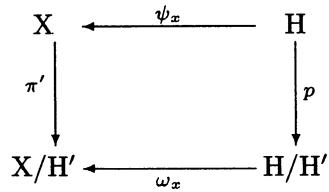
\includegraphics[keepaspectratio]{images/part001_c0ba5876.jpg}}

The mapping \((x,\xi)\mapsto\pi'(x\xi)\) of \(X\times H\) into \(X/H'\) is continuous; since \(\pi'(x\xi)=\pi'(x\xi\xi')\) for all \(\xi'\in H'\) this mapping defines, by passage to the quotient, a continuous mapping of \(X\times(H/H')\) into \(X/H'\) ; whence, for each fixed x in X, a partial mapping \(\omega_{x}\) of \(H/H'\) into \(X/H'\) , deduced by passage to the quotient from the mapping \(\psi_x: \xi \mapsto x\xi\) of H into X. Note that \(\psi_{x\xi} = \psi_x \circ \gamma_H(\xi)\) , therefore that \(\omega_{x\xi} = \omega_x \circ \gamma_{\mathrm{H/H'}}(\xi)\) for all \(\xi \in \mathrm{H}\) .

Lemma 7. --- Let K be a compact subset of X/H', and L a compact subset of X. Then \(\bigcup_{x\in\mathbf{L}}\omega_{x}^{-1}(\mathbf{K})\) is relatively compact in H/H'.

Let \(\mathbf{K}_1\) be a compact subset of \(\mathbf{X}\) such that \(\pi'(\mathbf{K}_1) = \mathbf{K}\) . Let \(\mathbf{K}_2\) be the set of \(\xi \in \mathbf{H}\) such that \(\mathbf{L}\xi\) intersects \(\mathbf{K}_1\) . Then \(\mathbf{K}_2\) is compact (GT, III, §4, No.~5, Th. 1). Let \(\xi \in \mathbf{H}\) be such that \(p(\xi) \in \bigcup_{x \in \mathbf{L}} \omega_x^{-1}(\mathbf{K})\) . Thus, there exists an \(x \in \mathbf{L}\) such that \(\omega_x(p(\xi)) \in \mathbf{K}\) , in other words such that \(\pi'(x\xi) \in \mathbf{K}\) . Since \(\pi'(\mathbf{K}_1) = \mathbf{K}\) , there exists \(\xi' \in \mathbf{H}'\) such that \(x\xi\xi' \in \mathbf{K}_1\) . Then \(\xi\xi' \in \mathbf{K}_2\) , therefore \(p(\xi) = p(\xi\xi') \in p(\mathbf{K}_2)\) . We have thus shown that \(\bigcup_{x \in \mathbf{L}} \omega_x^{-1}(\mathbf{K}) \subset p(\mathbf{K}_2)\) .

This lemma shows first of all that the mapping \(\omega_x\) is proper. One can therefore form the measure \(\omega_x(\beta/\beta')\) on \(\mathbf{X}/\mathbf{H}'\) , which is concentrated on \(\omega_x(\mathbf{H}/\mathbf{H}') = \pi'(\psi_x(\mathbf{H})) = \pi'(x\mathbf{H})\) . If \(f \in \mathcal{K}(\mathbf{X}/\mathbf{H}')\) , Lemma 7 and §1, No.~1, Lemma 1 show that the function \(x \mapsto \langle f, \omega_x(\beta/\beta') \rangle\) is continuous on \(\mathbf{X}\) ; moreover, \(\langle f, \omega_x(\beta/\beta') \rangle\) is zero when \(\operatorname{Supp} f\) does not intersect \(\pi'(x\mathbf{H})\) , in other words when \(\pi(x)\) does not belong to the canonical image of \(\operatorname{Supp} f\) in \(\mathbf{X}/\mathbf{H}\) .

Moreover, if \(x \in H\) then

\[
\omega_ {x \xi} (\beta / \beta^ {\prime}) = \omega_ {x} \left(\boldsymbol {\gamma} _ {\mathrm{H} / \mathrm{H} ^ {\prime}} (\xi) (\beta / \beta^ {\prime})\right) = \omega_ {x} (\beta / \beta^ {\prime}).
\]

The mapping \(x \mapsto \omega_x(\beta/\beta')\) of X into \(\mathcal{M}(\mathrm{X}/\mathrm{H}')\) therefore defines by passage to the quotient a mapping \(u \mapsto (\beta/\beta')_u\) of X/H into \(\mathcal{M}(\mathrm{X}/\mathrm{H}')\) . The foregoing shows that, for every \(f \in \mathcal{K}(\mathrm{X}/\mathrm{H}')\) , the mapping \(u \mapsto \langle f, (\beta/\beta')_u \rangle\) is continuous with compact support. Consequently the mapping \(u \mapsto (\beta/\beta')_u\) is a vaguely continuous and \((\mu/\beta)\) -adequate family of measures on \(\mathrm{X}/\mathrm{H}'\) , with \(\mathrm{X}/\mathrm{H}\) as index set.

Let \(x \in X\) , and \(u = \pi(x) \in X/H\) . Let \(f\) be a function on \(X/H'\) , with values in a Banach space or in \(\overline{R}\) . By Ch. V, §4, Th. 2, for \(f\) to be \((\beta/\beta')_u\) -integrable, it is necessary and sufficient that the function \(p(\xi) \mapsto f\big(\omega_x(p(\xi))\big) = f\big(\pi'(x\xi)\big)\) on \(H/H'\) be \((\beta/\beta')\) -integrable, in which case

\[
\int_ {\mathrm{X} / \mathrm{H} ^ {\prime}} \mathbf {f} (u ^ {\prime}) d (\beta / \beta^ {\prime}) _ {u} (u ^ {\prime}) = \int_ {\mathrm{H} / \mathrm{H} ^ {\prime}} \mathbf {f} \left(\pi^ {\prime} (x \xi)\right) d (\beta / \beta^ {\prime}) (\dot {\xi}) \quad \left(\dot {\xi} = p (\xi)\right).\tag{21}
\]

One has analogous properties for measurability, the upper integral and the essential integral.

PROPOSITION 12. --- With the foregoing notations,

\[
\int_ {\mathrm{X/H}} (\beta / \beta^ {\prime}) _ {u} d (\mu / \beta) (u) = \mu / \beta^ {\prime}.\tag{22}
\]

Let \(f \in \mathcal{K}(X)\) , and let \(f^{\flat} \in \mathcal{K}(X/H')\) , defined by

\[
f ^ {\flat} \left(\pi^ {\prime} (x)\right) = \int_ {\mathrm{H} ^ {\prime}} f \left(x \xi^ {\prime}\right) d \beta^ {\prime} \left(\xi^ {\prime}\right).
\]

It suffices (cf.~No.~2) to prove that \(f^{\flat}\) has the same integral with respect to the two members of (22). Now, \(\langle \mu / \beta', f^{\flat} \rangle = \langle \mu, f \rangle\) . On the other hand,

\[
\left\langle \int_ {\mathrm{X} / \mathrm{H}} \left(\beta / \beta^ {\prime}\right) _ {u} d (\mu / \beta) (u), f ^ {\flat} \right\rangle = \int_ {\mathrm{X} / \mathrm{H}} \left\langle \left(\beta / \beta^ {\prime}\right) _ {u}, f ^ {\flat} \right\rangle d (\mu / \beta) (u).
\]

Now, let \(x \in \mathbf{X}\) and \(u = \pi(x)\) . We have

\[
\begin{array}{r l} \langle (\beta / \beta^ {\prime}) _ {u}, f ^ {b} \rangle & = \langle \omega_ {x} (\beta / \beta^ {\prime}), f ^ {b} \rangle = \int_ {\mathrm{H/H} ^ {\prime}} f ^ {b} \big (\omega_ {x} (\dot {\xi}) \big) d (\beta / \beta^ {\prime}) (\dot {\xi}) \\ & = \int_ {\mathrm{H/H} ^ {\prime}} f ^ {b} \big (\pi^ {\prime} (x \xi) \big) d (\beta / \beta^ {\prime}) (\dot {\xi}) \\ & = \int_ {\mathrm{H/H} ^ {\prime}} d (\beta / \beta^ {\prime}) (\dot {\xi}) \int_ {\mathrm{H} ^ {\prime}} f (x \xi \xi^ {\prime}) d \beta^ {\prime} (\xi^ {\prime}) \\ & = \int_ {\mathrm{H}} f (x \xi) d \beta (\xi). \end{array}
\]

Therefore

\[
\left\langle \int_ {\mathrm{X/H}} (\beta / \beta^ {\prime}) _ {u} d (\mu / \beta) (u), f ^ {\flat} \right\rangle = \int_ {\mathrm{X/H}} d (\mu / \beta) (u) \int_ {\mathrm{H}} f (x \xi) d \beta (\xi) = \left\langle \mu , f \right\rangle ,
\]

which proves the proposition.

COROLLARY 1. --- a) Let f be a function on X/H', with values in a Banach space or in \(\overline{\mathbf{R}}\) , integrable for \(\mu/\beta'\) . There exists a \((\mu/\beta)\) -negligible subset N of X/H having the following property: if \(x \in X\) is such that \(\pi(x) \notin N\) , then the function \(\mathbf{f} \circ \omega_x\) on H/H', that is, the function \(\dot{\xi} \mapsto \mathbf{f}\big(\pi'(x\xi)\big)\) , is integrable for \(\beta/\beta'\) . The integral \(\int_{H/H'} \mathbf{f}\big(\pi'(x\xi)\big)d(\beta/\beta')(\dot{\xi})\) depends only on \(\dot{x} = \pi(x)\) , and is a \((\mu/\beta)\) -integrable function of \(\dot{x}\) ; and

\[
\int_ {\mathrm{X} / \mathrm{H} ^ {\prime}} \mathbf {f} d (\mu / \beta^ {\prime}) = \int_ {\mathrm{X} / \mathrm{H}} d (\mu / \beta) (\dot {x}) \int_ {\mathrm{H} / \mathrm{H} ^ {\prime}} \mathbf {f} \left(\pi^ {\prime} (x \xi)\right) d (\beta / \beta^ {\prime}) (\dot {\xi}).
\]

\begin{enumerate}
\def\labelenumi{\alph{enumi})}
\setcounter{enumi}{1}
\tightlist
\item
  Let \(f\) be a function \(\geqslant 0\) on \(\mathbf{X} / \mathbf{H}'\) , measurable for \(\mu / \beta'\) and zero outside a countable union of \((\mu / \beta')\) -integrable sets. Then
\end{enumerate}

\[
\pi (x) \mapsto \int_ {\mathrm{H} / \mathrm{H} ^ {\prime}} ^ {*} f (\pi^ {\prime} (x \xi)) d (\beta / \beta^ {\prime}) (\dot {\xi})
\]

is \((\mu /\beta)\) -measurable, and

\[
\int_ {\mathrm {X/ H^ {\prime}}} ^ {*} f d (\mu / \beta^ {\prime}) = \int_ {\mathrm{X/H}} ^ {*} d (\mu / \beta) (\dot {x}) \int_ {\mathrm {H/ H^ {\prime}}} ^ {*} f \bigl (\pi^ {\prime} (x \xi) \bigr) d (\beta / \beta^ {\prime}) (\dot {\xi}).
\]

\begin{enumerate}
\def\labelenumi{\alph{enumi})}
\setcounter{enumi}{2}
\tightlist
\item
  Let f be a function on X/H' with values in a Banach space or in \(\overline{R}\) , measurable for \(\mu/\beta'\) and zero outside a countable union of \((\mu/\beta')\) -integrable sets. Then, for f to be \((\mu/\beta')\) -integrable, it is sufficient that
\end{enumerate}

\[
\int_ {\mathrm{X} / \mathrm{H}} ^ {*} d (\mu / \beta) (\dot {x}) \int_ {\mathrm{H} / \mathrm{H} ^ {\prime}} ^ {*} | \mathbf {f} (\pi^ {\prime} (x \xi)) | d (\beta / \beta^ {\prime}) (\dot {\xi}) <   + \infty .
\]

COROLLARY 2. --- Let G be a locally compact group, A and B closed subgroups of G such that A ⊃ B. Suppose that there exists, on the homogeneous space G/B of left cosets with respect to B, a nonzero positive measure α that is invariant under G and is bounded.

\begin{enumerate}
\def\labelenumi{\alph{enumi})}
\item
  The canonical image of \(\alpha\) in \(\mathbf{G} / \mathbf{A}\) is a nonzero positive measure, invariant under \(\mathbf{G}\) , and bounded.
\item
  \(\Delta_{\mathrm{G}}\) coincides with \(\Delta_{\mathrm{A}}\) on A and with \(\Delta_{\mathrm{B}}\) on B.
\item
  There exists, on the homogeneous space A/B of left cosets of A with respect to B, a nonzero positive measure invariant under A and bounded.
\end{enumerate}

The assertion a) is immediate. The assertion b) follows from a) and No.~6, Cor. 2 of Th. 3. By b), \(\Delta_{\mathbf{A}}\) coincides with \(\Delta_{\mathbf{B}}\) on B, and one can therefore apply the results of the present subsection, on taking \(\mathbf{X} = \mathbf{G}\) , \(\mathbf{H} = \mathbf{A}\) , \(\mathbf{H}' = \mathbf{B}\) . The function 1 on \(\mathbf{G} / \mathbf{B}\) is \(\alpha\) -integrable. By a) of Cor. 1, the function 1 on \(\mathbf{A} / \mathbf{B}\) is integrable for \(\beta / \beta'\) , where \(\beta\) and \(\beta'\) denote left Haar measures on A and B; thus \(\beta / \beta'\) is bounded.

\subsection{Construction of the Haar measure of a group from the Haar measures of certain subgroups}

Let \(\mathbf{G}\) be a locally compact group, \(\mathbf{X}\) and \(\mathbf{Y}\) two closed subgroups of \(\mathbf{G}\) such that \(\Omega = \mathbf{XY}\) contains a neighborhood \(\mathbf{U}\) of \(e\) . Then \(\Omega\) is open in \(\mathbf{G}\) ; for, for any \(x_0 \in \mathbf{X}\) and \(y_0 \in \mathbf{Y}\) , \(\mathbf{XY} = (x_0\mathbf{X})(\mathbf{Y}y_0) \supset x_0\mathbf{U}y_0\) , and \(x_{0}Uy_{0}\) is a neighborhood of \(x_{0}y_{0}\) ; thus \(\Omega\) is a neighborhood of each of its points.

*When G is a Lie group with Lie algebra g, the condition imposed on X and Y is satisfied if the subalgebras corresponding to X and Y have sum g .*

The group \(X \times Y\) operates continuously in G on the left, by the law \((x, y) \cdot s = xsy^{-1}\) ( \(x \in X, y \in Y, s \in G\) ). Let \(Z = X \cap Y\) . The stabilizer of e in \(X \times Y\) is the subgroup \(Z_{0}\) of \(X \times Y\) formed by the pairs \((z, z)\) , where \(z \in Z\) , a subgroup canonically isomorphic to Z. Thus the set \(\Omega\) may be identified with the homogeneous space \((X \times Y)/Z_{0}\) of left cosets; more precisely, the mapping \((x, y) \mapsto xy^{-1}\) of \(X \times Y\) onto \(\Omega\) defines, by passage to the quotient, a continuous bijection of \((X \times Y)/Z_{0}\) onto \(\Omega\) . We shall assume that this mapping is a homeomorphism. (This is notably the case if G is countable at infinity: cf.~App. I.)

PROPOSITION 13. --- Suppose in addition that Z is compact. Let \(\mu_{\mathrm{G}}\) , \(\mu_{\mathrm{X}}\) , \(\mu_{\mathrm{Y}}\) be left Haar measures on G, X, Y, and \(\Lambda\) the restriction of \(\Delta_{\mathrm{G}}\) to Y. Then the restriction \(\mu\) of \(\mu_{\mathrm{G}}\) to \(\Omega\) is, up to a constant factor, the image of \(\mu_{\mathrm{X}} \otimes (\Lambda^{-1} \cdot \mu_{\mathrm{Y}})\) under the mapping \((x, y) \mapsto xy^{-1}\) of X × Y onto \(\Omega\) (a mapping that is proper).

For \(x\in \mathbf{X},y\in \mathbf{Y}\)

\[
\boldsymbol {\gamma} \big ((x, y) \big) \mu = \boldsymbol {\delta} (y) \boldsymbol {\gamma} (x) \mu = \Delta_ {G} (y) \mu .
\]

Identifying \(\Omega\) with the homogeneous space \((\mathrm{X} \times \mathrm{Y}) / \mathrm{Z}_0\) and choosing a suitable Haar measure on \(\mathbf{Z}_0\) , one sees that \(\mu^\sharp\) is the product of the left Haar measure of \(\mathrm{X} \times \mathrm{Y}\) , namely \(\mu_{\mathrm{X}} \otimes \mu_{\mathrm{Y}}\) , by the function \((x, y) \mapsto \Delta_{\mathrm{G}}(y)^{-1}\) (No.~6, Lemma 6). On the other hand \(\mu\) is, up to a constant factor, the image of \(\mu^\sharp\) under the canonical mapping of \(\mathrm{X} \times \mathrm{Y}\) onto \(\Omega\) (No.~3, Remark 2).

COROLLARY. --- Let f be a function defined on \(\Omega\) , with values in a Banach space or in \(\overline{R}\) . For f to be \(\mu\) -integrable, it is necessary and sufficient that the function \((x,y)\mapsto\mathbf{f}(xy)\Delta_{\mathrm{G}}(y)\Delta_{\mathrm{Y}}(y)^{-1}\) be \((\mu_{\mathrm{X}}\otimes\mu_{\mathrm{Y}})\) -integrable, in which case

\[
\int_ {\Omega} \mathbf {f} (\omega) d \mu (\omega) = a \iint_ {\mathrm{X} \times \mathrm{Y}} \mathbf {f} (x y) \Delta_ {\mathrm{G}} (y) \Delta_ {\mathrm{Y}} (y) ^ {- 1} d \mu_ {\mathrm{X}} (x) d \mu_ {\mathrm{Y}} (y),\tag{23}
\]

where \(a\) is a constant \(>0\) independent of \(\mathbf{f}\) .

By Prop. 13, and Ch. V, §4, No.~4, Th. 2, for f to be \(\mu\) -integrable, it is necessary and sufficient that the function \((x,y)\mapsto\mathbf{f}(xy^{-1})\) be integrable for \(\mu_{\mathrm{X}}\otimes(\Lambda^{-1}\cdot\mu_{\mathrm{Y}})\) , or again that the function \((x,y)\mapsto\mathbf{f}(xy^{-1})\Delta_{\mathrm{G}}(y)^{-1}\) be integrable for \(\mu_{X}\otimes\mu_{Y}\) , or again that the function \((x,y)\mapsto\mathbf{f}(xy)\Delta_{\mathrm{G}}(y)\Delta_{\mathrm{Y}}(y)^{-1}\) be integrable for \(\mu_{X}\otimes\mu_{Y}\) . Formula (23) results from an analogous argument.

PROPOSITION 14. --- Suppose that the conditions of Prop. 13 are fulfilled and that, in addition, Y is normal.

\begin{enumerate}
\def\labelenumi{\alph{enumi})}
\item
  The restriction of \(\mu_{\mathrm{G}}\) to \(\Omega\) is, up to a constant factor, the image of \(\mu_{\mathrm{X}} \otimes \mu_{\mathrm{Y}}\) under the mapping \((x,y) \mapsto xy\) of \(\mathrm{X} \times \mathrm{Y}\) onto \(\Omega\) .
\item
  For \(x \in \mathbf{X}\) and \(y \in \mathbf{Y}\) ,
\end{enumerate}

\[
\Delta_ {\mathrm{G}} (x y) = \Delta_ {\mathrm{X}} (x) \Delta_ {\mathrm{Y}} (y) \bmod (i _ {x}),
\]

where \(i_x\) denotes the automorphism \(v \mapsto x^{-1}vx\) of Y.

We have \(\Delta_{\mathrm{G}} = \Delta_{\mathrm{Y}}\) on Y (Prop. 10 b)), therefore a) follows from (23). Let \(x_0 \in \mathbf{X}\) , \(y_0 \in \mathbf{Y}\) . Denote by \(p\) the mapping \((x, y) \mapsto xy\) of \(\mathbf{X} \times \mathbf{Y}\) onto \(\Omega\) . Since

\[
x y \left(x _ {0} y _ {0}\right) ^ {- 1} = x x _ {0} ^ {- 1} \left(x _ {0} y y _ {0} ^ {- 1} x _ {0} ^ {- 1}\right) = x x _ {0} ^ {- 1} i _ {x _ {0} ^ {- 1}} \left(y y _ {0} ^ {- 1}\right),
\]

we have

\[
\begin{array}{r l} \Delta_ {\mathrm{G}} (x _ {0} y _ {0}) p (\mu_ {\mathrm{X}} \otimes \mu_ {\mathrm{Y}}) & = \pmb {\delta} (x _ {0} y _ {0}) p (\mu_ {\mathrm{X}} \otimes \mu_ {\mathrm{Y}}) \\ & = p \big (\pmb {\delta} (x _ {0}) \mu_ {\mathrm{X}} \otimes i _ {x _ {0} ^ {- 1}} \pmb {\delta} (y _ {0}) \mu_ {\mathrm{Y}} \big) \\ & = p \big (\Delta_ {\mathrm{X}} (x _ {0}) \mu_ {\mathrm{X}} \otimes \Delta_ {\mathrm{Y}} (y _ {0}) (\bmod i _ {x _ {0}}) \mu_ {\mathrm{Y}} \big) \\ & = \Delta_ {\mathrm{X}} (x _ {0}) \Delta_ {\mathrm{Y}} (y _ {0}) (\bmod i _ {x _ {0}}) p (\mu_ {\mathrm{X}} \otimes \mu_ {\mathrm{Y}}), \end{array}
\]

whence b).

Remark. --- Prop. 14 applies in particular when G is the topological semi-direct product of X by Y (GT, III, §2, No.~10). In this case, \(Z = \{e\}\) and \(\Omega = G\) . Since \(yx = x i_{x}(y)\) for \(x \in X\) , \(y \in Y\) , the measure \(\mu_{G}\) is also, up to a constant factor, the image of \((\text{mod } i_{x})\mu_{X} \otimes \mu_{Y}\) under the mapping \((x, y) \mapsto yx\) of \(X \times Y\) into G.

\subsection{Integration on a fundamental domain}

Let X be a locally compact space, H a discrete group operating on the right continuously and properly in X. Let \(\pi\) be the canonical mapping of X onto X/H. For every \(x \in X\) , we denote by \(H_x\) the stabilizer of x in H; this is a finite subgroup of H (GT, III, §4, No.~2, Prop. 4); its order will be denoted \(n(x)\) . For every \(s \in H\) , \(H_{xs} = s^{-1}H_x s\) , therefore \(n(xs) = n(x)\) . There exists an open neighborhood U of x such that \(U \cap Us = \varnothing\) for \(s \notin H_x\) (loc. cit., No.~4, proof of Prop. 8); for \(y \in U\) , one has \(H_y \subset H_x\) ; thus the function n on X is upper semi-continuous. When X is countable at infinity, H is countable; for, let \((\mathrm{K}_1, \mathrm{K}_2, \ldots)\) be a covering of X by a sequence of compact subsets, and let \(x_{0} \in X\) ; the set of \(s \in H\) such that \(x_{0}s \in K_{i}\) is finite (loc. cit., No.~5, Th. 1), whence our assertion.

DEFINITION 2. --- Let \(F \subset X\) . One says that F is a fundamental domain (for H) if the restriction of \(\pi\) to F is a bijection of F onto X/H (in other words, F is a system of representatives for the equivalence relation defined by H).

Lemma 8. --- Let F be a fundamental domain. For every \(x \in \mathbf{X}\) ,

\[
\sum_ {s \in \mathrm{H}} \varphi_ {\mathrm{F} s} (x) = n (x).\tag{24}
\]

Since \(\varphi_{\mathrm{Fs}}(xt) = \varphi_{\mathrm{Fst}^{-1}}(x)\) for all \(s\) and \(t\) in \(\mathbf{H}\) , the two members of (24) remain invariant when \(x\) is replaced by \(xt\) . We can therefore suppose that \(x \in \mathbf{F}\) . We then have the equivalences

\[
\varphi_ {\mathrm{Fs}} (x) = 1 \Leftrightarrow x \in \mathrm{Fs} \Leftrightarrow x s ^ {- 1} \in \mathrm{F} \Leftrightarrow x s ^ {- 1} = x \Leftrightarrow s \in \mathrm{H} _ {x},
\]

whence (24).

PROPOSITION 15. --- Assume that X is countable at infinity. Let \(\mu\) be a measure \(\geqslant 0\) on X. Let F be a fundamental domain such that Fs is \(\mu\) -measurable for every \(s \in H\) . Let f be a \(\mu\) -integrable function on X, with values in a Banach space or in \(\overline{\mathbf{R}}\) . Then the family of the

\[
\int_ {\mathrm{Fs}} n (x) ^ {- 1} \mathbf {f} (x) d \mu (x) \quad (s \in \mathbf {H})
\]

is summable, and

\[
\int_ {\mathrm{X}} \mathbf {f} (x) d \mu (x) = \sum_ {s \in \mathrm{H}} \int_ {\mathrm{F} s} n (x) ^ {- 1} \mathbf {f} (x) d \mu (x).
\]

If \(\mathbf{A}\) is a finite subset of \(\mathbf{H}\) , then

\[
\left| \sum_ {s \in \mathrm{A}} n ^ {- 1} \mathbf {f} \varphi_ {\mathrm{Fs}} \right| \leqslant n ^ {- 1} | \mathbf {f} | \sum_ {s \in \mathrm{A}} \varphi_ {\mathrm{Fs}} \leqslant | \mathbf {f} |
\]

by Lemma 8. Lemma 8 also proves that \(\sum_{s\in\mathbf{A}}n^{-1}\mathbf{f}\varphi_{\mathrm{F}s}\) converges pointwise to \(\mathbf{f}\) with respect to the increasing directed set of finite subsets of \(\mathbf{H}\) . Prop. 15 then follows from Ch. IV, §4, No.~3, Th. 2.

THEOREM 4. --- Let X be a locally compact space countable at infinity, H a discrete group operating continuously and properly on the right in X, \(\pi\) the canonical mapping of X onto X/H, \(\mu\) a positive measure on X invariant under H, \(\beta\) the normalized Haar measure of H, and \(\lambda = \mu/\beta\) . Let F be a \(\mu\) -measurable fundamental domain.

\begin{enumerate}
\def\labelenumi{\alph{enumi})}
\tightlist
\item
  The pair \((\pi, n^{-1}\varphi_{\mathrm{F}})\) is \(\mu\) -adapted, and
\end{enumerate}

\[
\int_ {\mathrm{X}} n (x) ^ {- 1} \varphi_ {\mathrm{F}} (x) \varepsilon_ {\pi (x)} d \mu (x) = \lambda .
\]

\begin{enumerate}
\def\labelenumi{\alph{enumi})}
\setcounter{enumi}{1}
\item
  The mapping \(\pi\) is proper for \(n^{-1}\varphi_{\mathrm{F}}\cdot \mu\) , and \(\pi (n^{-1}\varphi_{\mathrm{F}}\cdot \mu) = \lambda\) .
\item
  Let k be a function on X/H. For k to be \(\lambda\) -measurable (resp. \(\lambda\) -integrable), it is necessary and sufficient that \(n^{-1}\varphi_{\mathrm{F}}(k\circ\pi)\) be \(\mu\) -measurable (resp. \(\mu\) -integrable); and, if k is \(\lambda\) -integrable then
\end{enumerate}

\[
\int_ {\mathrm{X/H}} k d \lambda = \int_ {\mathrm{F}} n ^ {- 1} (k \circ \pi) d \mu .
\]

We have \(\mu = \lambda^{\sharp}\) . Let \(f \in \mathcal{H}_{+}(\mathrm{X / H})\) . Then \(n^{-1}\varphi_{\mathrm{F}}(f \circ \pi)\) is \(\mu\) -measurable and \(\geqslant 0\) , and by Prop. 5 b) of No.~3 we have

\[
\int_ {\mathrm{X}} ^ {*} n (x) ^ {- 1} \varphi_ {\mathrm{F}} (x) f (\pi (x)) d \mu (x) = \int_ {\mathrm{X/H}} ^ {*} f (\dot {x}) d \lambda (\dot {x}) \int_ {\mathrm{H}} ^ {*} n (x \xi) ^ {- 1} \varphi_ {\mathrm{F}} (x \xi) d \beta (\xi)
\]

and \(\int_{\mathrm{H}}^{*}n(x\xi)^{-1}\varphi_{\mathrm{F}}(x\xi)d\beta (\xi) = n(x)^{-1}\sum_{\xi \in \mathrm{H}}\varphi_{\mathrm{F}}(x\xi) = 1\) by Lemma 8. Thus \(n^{-1}\varphi_{\mathrm{F}}\cdot (f\circ \pi)\) is \(\mu\) -integrable and

\[
\int_ {\mathrm{X}} n (x) ^ {- 1} \varphi_ {\mathrm{F}} (x) f (\pi (x)) d \mu (x) = \int_ {\mathrm{X/H}} f (\dot {x}) d \lambda (\dot {x}).
\]

This proves a). The assertion b) is proved similarly. The assertion c) may be deduced from a) and from Ch. V, §4, Prop. 3 and Th. 2.

COROLLARY. --- We maintain the hypotheses and notations of Th. 4. Let F' be a second μ-measurable fundamental domain. Let u be a function on X, with values in a Banach space or in \(\overline{R}\) , invariant under H. Suppose that u is μ-integrable on F. Then u is μ-integrable on F' and

\[
\int_ {\mathrm{F}} \mathbf {u} (x) d \mu (x) = \int_ {\mathrm{F} ^ {\prime}} \mathbf {u} (x) d \mu (x).
\]

Since \(\mathbf{u}\) and \(n\) are invariant under \(\mathbf{H}\) , there exists a function \(\mathbf{v}\) on \(\mathrm{X / H}\) such that \(\mathbf{v} \circ \pi\) coincides with \(n\mathbf{u}\) on \(\mathbf{F}\) and on \(\mathbf{F}'\) . Then \(n^{-1}\varphi_{\mathrm{F}}(\mathbf{v}\circ \pi) = \varphi_{\mathrm{F}}\mathbf{u}, n^{-1}\varphi_{\mathrm{F}^{\prime}}(\mathbf{v}\circ \pi) = \varphi_{\mathrm{F}^{\prime}}\mathbf{u}.\) By hypothesis, \(n^{-1}\varphi_{\mathrm{F}}(\mathbf{v}\circ \pi)\) is \(\mu\) -integrable. By Th. 4, \(\mathbf{v}\) is \(\lambda\) -integrable, \(\varphi_{\mathrm{F}^{\prime}}\mu\) is \(\mu\) -integrable, and

\[
\int_ {\mathrm{F}} \mathbf {u} d \mu = \int_ {\mathrm{X/H}} \mathbf {v} d \lambda = \int_ {\mathrm{F} ^ {\prime}} \mathbf {u} d \mu .
\]

For the existence of \(\mu\) -measurable fundamental domains, see Exer. 12.

\section{APPLICATIONS AND EXAMPLES}

\subsection{Compact groups of linear mappings}

Let E be a finite-dimensional vector space over R, C or H. Then End(E) is a finite-dimensional algebra over R, and the canonical topology on End(E) (§1, No.~10) is the topology of compact convergence. The group \(\operatorname{Aut}(E) = \mathbf{GL}(E)\) is an open subset of End(E), hence is a locally compact group. Let \((e_{1}, e_{2}, \ldots, e_{n})\) be a basis of E and, for every endomorphism u of E, let \(M(u) = (\alpha_{ij}(u))\) be the matrix of u with respect to this basis; to say that a subset S of End(E) is relatively compact in End(E) is equivalent to saying that the functions \(\alpha_{ij}(u)\) are bounded in S.

PROPOSITION 1. --- Let G be a subgroup of Aut(E). The following three properties are equivalent:

\begin{enumerate}
\def\labelenumi{(\roman{enumi})}
\item
  G is relatively compact in \(\operatorname{End}(\mathbf{E})\) ;
\item
  G is relatively compact in \(\operatorname{Aut}(\mathbf{E})\) ;
\item
  G leaves invariant a nondegenerate \(^{1}\) positive hermitian form on E. (iii) \(\Rightarrow\) (i): Suppose that G leaves invariant a nondegenerate positive hermitian form \(\Psi\) . Let \((e_{1},\ldots,e_{n})\) be an orthonormal basis for \(\Psi\) (Alg., Ch. IX, §6, No.~1, Cor. 1 of Th. 1). For every \(u\in G\) , let \((u_{ij})\) be its matrix with respect to \((e_{i})\) . For any j, we have \(\sum_{i=1}^{n}|u_{ij}|^{2}=1\) , thus \(|u_{ij}|\leqslant1\) for all i and j, which proves (i).
\item
  \(\Rightarrow\) (ii): This follows from GT, X, §3, No.~5, Cor. of Th. 4, taking into account the fact that the topology of \(\operatorname{End}(\mathbf{E})\) is that of compact convergence.
\item
  \(\Rightarrow\) (iii): Suppose that the closure \(\overline{\mathbf{G}}\) of \(\mathbf{G}\) in \(\operatorname{Aut}(\mathbf{E})\) is compact. Let \(\Phi\) be a nondegenerate positive hermitian form on \(\mathbf{E}\) . If the field of scalars is \(\mathbf{R}\) or \(\mathbf{C}\) , the giving of \(\Phi\) makes \(\mathbf{E}\) a finite-dimensional Hilbert space, and condition (iii) will result from the following lemma:
\end{enumerate}

Lemma 1. --- Let F be a Hilbert space, K a compact group, and \(s \mapsto U(s)\) a representation of K in the group of invertible elements of \(\mathcal{L}(\mathrm{F};\mathrm{F})\) , continuous for the topology of pointwise convergence. There exists a nondegenerate positive hermitian form \(\varphi\) on F such that

\[
\varphi (U (s) x, U (s) y) = \varphi (x, y)
\]

for all \(s \in \mathbf{K}\) , \(x \in \mathbf{F}\) , \(y \in \mathbf{F}\) , and such that the topological vector space structure of \(\mathbf{F}\) defined by \(\varphi\) (TVS, V, §1, No.~3) is identical to the original structure of \(\mathbf{F}\) .

Let \(\alpha\) be a Haar measure on \(\mathbf{K}\) . For any \(x, y\) in \(\mathbf{F}\) , the mapping \(s \mapsto (U(s)x|U(s)y)\) is continuous. Set

\[
\varphi (x, y) = \int (U (s) x | U (s) y) d \alpha (s).
\]

It is immediate that \(\varphi(x,y)\) is a sesquilinear form on \(\mathbf{F}\) . Since the set of endomorphisms \(U(s)\) is compact in \(\mathcal{L}_s(\mathrm{F};\mathrm{F})\) , there exists a constant \(\mathbf{M}\) such that \(\| U(s)\| \leqslant \mathbf{M}\) for all \(s\in \mathbf{K}\) . For every \(x\in \mathbf{F}\) , we therefore have

\[
\mathrm{M} ^ {- 1} \| x \| \leqslant \| U (s) x \| \leqslant \mathrm{M} \| x \|,
\]

whence the inequalities

\[
\mathbf {M} ^ {- 2} \alpha (\mathbf {K}) \| x \| ^ {2} \leqslant \varphi (x, x) \leqslant \mathbf {M} ^ {2} \alpha (\mathbf {K}) \| x \| ^ {2},
\]

which shows that \(\varphi\) is positive and nondegenerate, and that the norm \(\varphi(x,x)^{1/2}\) is equivalent to the norm \(\|x\|\) . Finally, for all \(t \in K\) ,

\[
\begin{array}{r l} & {\varphi (U (t) x, U (t) y) = \int (U (s t) x | U (s t) y) d \alpha (s)} \\ & {\qquad = \int (U (s) x | U (s) y) d \alpha (s) = \varphi (x, y).} \end{array}
\]

When the field of scalars is H, one argues exactly as before on replacing everywhere the function \(s \mapsto (U(s)x|U(s)y)\) by the function \(s \mapsto \Phi(sx, sy)\) defined on G, with values in H. This completes the proof of the proposition.

Remark. --- Let \(\Phi\) be a nondegenerate positive hermitian form on E. The unitary group \(\mathbf{U}(\Phi)\) is closed in \(\operatorname{Aut}(\mathbf{E})\) , hence is compact (Prop. 1). Prop. 1 also shows that every compact subgroup of \(\operatorname{Aut}(\mathbf{E})\) is contained in a subgroup of the form \(\mathbf{U}(\Phi)\) . If now \(\mathbf{U}(\Phi)\) is contained in a compact subgroup K of \(\operatorname{Aut}(\mathbf{E})\) , one sees that there exists a nondegenerate positive hermitian form \(\Phi'\) on E such that \(\mathbf{U}(\Phi) \subset \mathbf{K} \subset \mathbf{U}(\Phi')\) , and it follows easily (Exer. 1) that \(\Phi\) and \(\Phi'\) are proportional, whence \(\mathbf{U}(\Phi) = K\) . Thus the maximal compact subgroups of \(\operatorname{Aut}(E)\) are the subgroups of the form \(\mathbf{U}(\Phi)\) .

\subsection{Triviality of fibered spaces and of group extensions}

PROPOSITION 2. --- Let X be a locally compact space in which a locally compact group H acts on the right, continuously and properly, by \((x,\xi)\mapsto x\xi\) . Assume that X/H is paracompact. Let g be a continuous representation of H in \(R^{n}\) . Then there exists a continuous mapping f of X into \(R^{n}\) such that \(f(x\xi)=f(x)+g(\xi)\) for all \(x\in X\) and \(\xi\in H\) .

One reduces immediately to the case that n = 1. Since the additive group R is isomorphic to the multiplicative group \(R_{+}^{*}\) , the proposition is then an immediate consequence of Prop. 7 of §2, No.~4.

COROLLARY. --- Let X be a locally compact space in which a finite-dimensional real vector space V operates on the right, continuously and properly, by \((x,v)\mapsto xv\) . Let \(\pi\) be the canonical mapping of X onto B = X/V. Assume that B is paracompact.

\begin{enumerate}
\def\labelenumi{\alph{enumi})}
\item
  There exists a continuous mapping \(f\) of \(\mathbf{X}\) into \(\mathbf{V}\) such that \(f(xv) = f(x) + v\) for all \(x \in \mathbf{X}\) and \(v \in \mathbf{V}\) .
\item
  If \(f\) is a mapping satisfying the conditions of a), then the mapping \(x \mapsto (\pi(x), f(x))\) is a homeomorphism of \(X\) onto \(B \times V\) .
\end{enumerate}

The assertion a) results from Prop. 2 in which g is taken to be the identity mapping of V. Let f be a mapping satisfying the conditions of a). The mapping \(x \mapsto x \cdot (-f(x))\) of X into X is continuous, and is constant on each orbit, hence is of the form \(\varphi \circ \pi\) , where \(\varphi\) is a continuous mapping of B into X; for every \(b \in B\) , \(\pi(\varphi(b)) = b\) . The mappings \(x \mapsto (\pi(x), f(x))\) of X into B × V and \((b, v) \mapsto \varphi(b) \cdot v\) of B × V into X are inverse to each other, because \(\varphi(\pi(x)) \cdot f(x) = x \cdot (-f(x)) \cdot (f(x)) = x\) , \(\pi(\varphi(b) \cdot v) = \pi(\varphi(b)) = b\) , and, if \(b = \pi(y)\) , then

\[
f (\varphi (\pi (y)) \cdot v) = f (y \cdot (- f (y)) \cdot v) = f (y) - f (y) + v = v.
\]

Since these mappings are continuous, they are homeomorphisms.

Remark. --- Let E be a finite-dimensional real affine space, T a compact space, \(\mu\) a measure on T of total mass 1, and f a continuous mapping of T into E. If an origin a in E is chosen, E becomes equipped with a vector space structure, and the integral \(\int_{\mathrm{T}} f(t) d\mu(t)\) therefore has meaning; it represents the point x of E such that

\[
x - a = \int_ {\mathrm{T}} (f (t) - a) d \mu (t).
\]

This point is independent of the choice of \(a\) . For, let \(a' \in \mathbf{E}\) and \(x' \in \mathbf{E}\) be such that \(x' - a' = \int_{\mathbf{T}} (f(t) - a') d\mu(t)\) . Then

\[
\begin{array}{c} x ^ {\prime} - a = (x ^ {\prime} - a ^ {\prime}) + (a ^ {\prime} - a) = \int_ {\mathrm{T}} \bigl (f (t) - a ^ {\prime} \bigr) d \mu (t) + \int_ {\mathrm{T}} (a ^ {\prime} - a) d \mu (t) \\ = \int_ {\mathrm{T}} \bigl (f (t) - a \bigr) d \mu (t) = x - a, \end{array}
\]

whence \(x' = x\) . We may therefore employ the symbol \(\int_{\mathrm{T}} f(t) d\mu(t)\) without specifying the choice of origin in E. If u is an affine mapping of E into another finite-dimensional affine space \(E'\) , then

\[
u \Big (\int_ {\mathrm{T}} f (t) d \mu (t) \Big) = \int_ {\mathrm{T}} u \big (f (t) \big) d \mu (t).
\]

For, E and \(E'\) may be identified with vector spaces in such a way that u becomes a linear mapping, in which case the formula is known (Ch. III, §3, No.~2, Prop. 2 and No.~3, Prop. 7).

Lemma 2. --- Let G be a compact group, \(\mu\) the normalized Haar measure of G, E a finite-dimensional real affine space, A the affine group of E, and \(\rho\) a homomorphism of G into A. Assume that, for every \(x \in \mathbf{E}\) , the mapping \(s \mapsto \rho(s)x\) of G into E is continuous. Then, for every \(x \in \mathbf{E}\) , the point

\[
x _ {0} = \int_ {\mathrm{G}} \rho (s) x d \mu (s) \in \mathrm{E}
\]

is invariant under G.

For, for every \(t \in G\) ,

\[
\rho (t) x _ {0} = \int_ {\mathrm{G}} \rho (t) \rho (s) x d \mu (s) = \int_ {\mathrm{G}} \rho (t s) x d \mu (s) = \int_ {\mathrm{G}} \rho (s) x d \mu (s) = x _ {0}.
\]

PROPOSITION 3. --- Let G be a locally compact group. Let H be a closed normal subgroup of G, isomorphic to \(\mathbf{R}^n\) and such that \(\mathbf{G} / \mathbf{H}\) is compact.

\begin{enumerate}
\def\labelenumi{\alph{enumi})}
\item
  There exists a closed subgroup \(\mathbf{L}\) of \(\mathbf{G}\) such that \(\mathbf{G}\) is the topological semi-direct product of \(\mathbf{L}\) and \(\mathbf{H}\) .
\item
  If \(\mathbf{M}\) is a compact subgroup of \(\mathbf{G}\) , there exists an element \(x \in \mathbf{H}\) such that \(x^{-1}\mathbf{M}x \subset \mathbf{L}\) .
\item
  Every compact subgroup of \(\mathbf{G}\) is contained in a maximal compact subgroup.
\item
  The maximal compact subgroups of \(\mathbf{G}\) are the subgroups that are the transforms of \(\mathbf{L}\) by the inner automorphisms of \(\mathbf{G}\) .
\end{enumerate}

Let \(\pi\) be the canonical homomorphism of \(\mathbf{G}\) onto \(\mathbf{K} = \mathbf{G} / \mathbf{H}\) . By passage to the quotient, the mapping \((s,h)\mapsto shs^{-1}\) of \(\mathbf{G}\times \mathbf{H}\) into \(\mathbf{H}\) defines a continuous mapping \((\sigma ,h)\mapsto \sigma \cdot h\) of \(\mathbf{K}\times \mathbf{H}\) into \(\mathbf{H}\) such that \(shs^{-1} = \pi (s)\cdot h\) . We shall identify \(\mathbf{H}\) with \(\mathbf{R}^n\) (and will therefore employ, as the case may be, either the multiplicative or the additive notation for the group law in \(\mathbf{H}\) ). By the Cor. of Prop. 2, there exists a continuous mapping \(f\) of \(\mathbf{G}\) into \(\mathbf{H}\) such that \(f(xh) = f(x) + h\) for \(x\in \mathbf{G}, h\in \mathbf{H}\) . For every \(x\in \mathbf{G}\) , let \(p(x) = x\cdot (-f(x))\) , which depends only on the coset of \(x\) with respect to \(\mathbf{H}\) . Set

\[
\begin{array}{r l} \mathrm{F} (x, y) & = p (x y) ^ {- 1} p (x) p (y) = f (x y) y ^ {- 1} x ^ {- 1} x (- f (x)) y (- f (y)) \\ & = f (x y) [ y ^ {- 1} (- f (x)) y ] (- f (y)) \\ & = f (x y) - \pi (y) ^ {- 1} f (x) - f (y). \end{array}\tag{1}
\]

We see that if \(F(x,y) = 0\) for all x,y in G, then \(p(G) = L\) is a subgroup of G that intersects each coset of H in one and only one point. Since p is continuous, G is then the topological semi-direct product of L and H (GT, III, §2, No.~10).

Now, for any \(h, h' \in H\) ,

\[
\begin{array}{r l} F (x h, y h ^ {\prime}) & = f (x h y h ^ {\prime}) - \pi (y) ^ {- 1} f (x h) - f (y h ^ {\prime}) \\ & = f (x h y) + h ^ {\prime} - \pi (y) ^ {- 1} f (x) - \pi (y) ^ {- 1} h - f (y) - h ^ {\prime} \\ & = f \big (x y (\pi (y) ^ {- 1} h) \big) - \pi (y) ^ {- 1} f (x) - f (y) - \pi (y) ^ {- 1} h \\ & = f (x y) - \pi (y) ^ {- 1} f (x) - f (y) = F (x, y). \end{array}
\]

Therefore F defines, by passage to quotients, a continuous mapping \(\varphi\) of \(K \times K\) into H.

On the other hand, for all \(x, y, z\) in \(\mathbf{G}\) , we have

\[
\begin{array}{r l} & {\mathrm{F} (z, x y) + \mathrm{F} (x, y) = f (z x y) - \pi (x y) ^ {- 1} f (z) - f (x y) + f (x y)} \\ & {\qquad - \pi (y) ^ {- 1} f (x) - f (y)} \\ & {\qquad = \pi (y) ^ {- 1} f (z x) - \pi (x y) ^ {- 1} f (z) - \pi (y) ^ {- 1} f (x) + f (z x y)} \\ & {\qquad - \pi (y) ^ {- 1} f (z x) - f (y)} \\ & {\qquad = \pi (y) ^ {- 1} \mathrm{F} (z, x) + \mathrm{F} (z x, y),} \end{array}
\]

therefore, for all \(x', y', z'\) in \(\mathbf{K}\) ,

\[
- \varphi (x ^ {\prime}, y ^ {\prime}) = \varphi (z ^ {\prime}, x ^ {\prime} y ^ {\prime}) - y ^ {- 1} \varphi (z ^ {\prime}, x ^ {\prime}) - \varphi (z ^ {\prime} x ^ {\prime}, y ^ {\prime}).
\]

Let us integrate with respect to \(z'\) by means of the normalized Haar measure \(\alpha\) of K. Setting \(\psi(x') = \int \varphi(z', x') d\alpha(z')\) , \(\psi\) is a continuous function on K, and (on observing that the operations of K in \(R^{n}\) respect the vector space structure of \(R^{n}\) by GT, VII, §2, No.~1, Prop. 1), one obtains

\[
- \varphi (x ^ {\prime}, y ^ {\prime}) = \psi (x ^ {\prime} y ^ {\prime}) - y ^ {- 1} \psi (x ^ {\prime}) - \psi (y ^ {\prime}).
\]

In other words, setting \(k - \psi \circ \pi\) , which is a continuous function on G,

\[
- \mathrm{F} (x, y) = k (x y) - \pi (y) ^ {- 1} k (x) - k (y).\tag{2}
\]

Comparing (1) and (2), one sees that if \(f\) is replaced by the continuous function \(f + k\) (which leaves verified the property \(f(xh) = f(x) + h\) ), \(F\) is replaced by 0 and, as we saw earlier, this completes the proof of a).

For every \(g \in \mathbf{G}\) , let \(l_g\) (resp. \(h_g\) ) be the unique element of \(\mathbf{L}\) (resp. \(\mathbf{H}\) ) such that \(g = h_g l_g\) . If \(h_1 \in \mathbf{H}\) and \(g \in \mathbf{G}\) , then

\[
g h _ {1} = h _ {g} l _ {g} h _ {1} = h _ {g} (l _ {g} h _ {1} l _ {g} ^ {- 1}) l _ {g},
\]

thus \(h_{gh_1} = h_g + l_g h_1 l_g^{-1}\) . For every \(g \in \mathbf{G}\) , let \(\psi_g\) be the mapping of \(\mathbf{H}\) into itself defined by

\[
\psi_ {g} (h _ {1}) = h _ {g} + l _ {g} h _ {1} l _ {g} ^ {- 1}.
\]

One sees that the mapping \((g,h_{1})\mapsto\psi_{g}(h_{1})\) of G×H into H is continuous and makes H a homogeneous space for G, in which the stabilizer of the origin is L. We observe moreover that when H is identified with \(R^{n}\) , \(\psi_{g}\) is an affine mapping of H into itself. This said, let M be a compact subgroup of G; by Lemma 2, there exists an \(x\in H\) such that \(\psi_{m}(x)=x\) for all \(m\in M\) . For \(y\in H\) , \(\psi_{y}\) is the translation with vector y; it follows that for every \(m\in M\) , \(\psi_{x^{-1}}\circ\psi_{m}\circ\psi_{x}\) transforms the origin of H into itself, therefore \(x^{-1}mx\in L\) . This proves that \(x^{-1}Mx\subset L\) , whence b).

Let \(L'\) be a closed subgroup of \(G\) containing \(L\) . Then \(L'\) is the topological semi-direct product of \(L\) and \(L' \cap H\) . If \(L'\) is compact, then \(L' \cap H\) is compact hence reduces to a point (GT, IV, §2, No.~2, Cor. 1 of Th. 2), therefore \(L' = L\) . This proves that \(L\) is a maximal compact subgroup of \(G\) ; the same is therefore true of the subgroups that are the transforms of \(L\) by the inner automorphisms of \(G\) . The assertions c) and d) of Prop. 3 are then immediate consequences of b).

PROPOSITION 4. --- Let G be a locally compact group and H a closed normal subgroup of G such that K = G/H is compact. Then every continuous representation u of H in R, such that \(u(s\xi s^{-1}) = u(\xi)\) for all \(\xi \in H\) and \(s \in G\) , may be extended to a continuous representation of G in R.

Let \(L = G \times R\) and let M be the set of \((\xi, -u(\xi))\) , where \(\xi\) runs over H. It is clear that M is a closed normal subgroup of L. Let \(L' = L/M\) and let \(\pi\) be the canonical mapping of L onto \(L'\) . The subgroup of L generated by M and R is \(H \times R\) , hence is closed; therefore \(\pi(\mathbf{R})\) is a closed subgroup N of \(L'\) . The restriction \(\rho\) of \(\pi\) to R is a bijective continuous representation of R onto N. Lemma 2 of Appendix 1 proves that \(\rho\) is bicontinuous. Moreover, \(L'/N\) is isomorphic to \(\mathrm{L}/(\mathrm{H} \times \mathbf{R}) = \mathrm{G}/\mathrm{H}\) , hence is compact. By Prop. 3, and taking into account the fact that N is in the center of \(L'\) , \(L'\) is the product of N with another subgroup. Therefore there exists a continuous representation of \(L'\) onto N that reduces on N to the identity mapping. Therefore there exists a continuous representation v of L onto R that is trivial on M and reduces on R to the identity mapping. For \(\xi \in H\) , one has \(v((\xi,0)) = v((\xi,-u(\xi))(e,u(\xi))) = u(\xi)\) , which completes the proof.

Lemma 3. --- Let G be a topological group generated by a compact neighborhood of e. Let H be a closed subgroup of G such that the homogeneous space G/H is compact. Then H is generated by a compact neighborhood of e in H.

Let C be a compact set such that G = CH. Enlarging C if necessary, we can suppose that C generates G and that G = \(\overset{\circ}{CH}\) . Then \(C^{2}\) is compact and is covered by the \(\overset{\circ}{Cs}\) ( \(s \in H\) ), which are open. Therefore there exist \(s_{1}, \ldots, s_{n}\) in H such that \(C^{2} \subset \overset{\circ}{Cs}_{1} \cup \cdots \cup \overset{\circ}{Cs}_{n}\) . Let \(\Gamma\) be the subgroup of H generated by the \(s_{i}\) . Then \(C^{2} \subset \mathrm{C}\Gamma\) . By induction, it follows that \(C^{n} \subset \mathrm{C}\Gamma\) for every n, therefore G = C \(\Gamma\) . Every element of H may be put in the form ab with \(a \in C\) , \(b \in \Gamma\) , whence \(a \in H\) , whence \(a \in C \cap H\) . Therefore H is generated by \(C \cap H\) and the \(s_{i}\) , that is, by a compact set.

Lemma 4. --- Let G be a connected topological group, D a totally disconnected normal subgroup of G. Then D is contained in the center of G.

For, let \(d \in \mathbf{D}\) . The image of \(\mathbf{G}\) under the continuous mapping \(x \mapsto x dx^{-1}\) is a connected subset of \(\mathbf{D}\) , hence reduces to \(\{d\}\) , which proves that \(xd = dx\) for all \(x \in \mathbf{G}\) .

PROPOSITION 5. --- Let G be a connected topological group admitting a discrete normal subgroup D such that K = G/D is compact, and such that the commutator subgroup of K is dense in K. Then D is finite and G is compact.

The group G is locally isomorphic to K (GT, III, §2, No.~6, Prop. 19), hence is locally compact; since it is connected, it is generated by a compact neighborhood of e. By Lemmas 3 and 4, D is a finitely generated abelian group, hence is isomorphic to a group \(Z^{r} \times D_{1}\) with \(D_{1}\) finite (A, VII, §4, No.~7, Th. 3). Suppose that r \textgreater{} 0. Then there exists a representation f of D onto Z. By Prop. 4, f may be extended to a continuous representation g of G in R. By passage to quotients, g defines a continuous representation \(g'\) of K in R/Z; since R/Z is abelian, the kernel of \(g'\) contains the commutator subgroup of K, therefore \(g'\) is trivial; in other words, \(g(\mathbf{G}) \subset \mathbf{Z}\) . Since G is connected, it follows that \(g(\mathbf{G}) = \{0\}\) , which is absurd since \(f(\mathbf{D}) = \mathbf{Z}\) . Thus r = 0 and D is finite. Consequently G is compact (GT, III, §4, No.~1, Cor. 2 of Prop. 2).
